\chapter{Data Samples and Physics Objects}
\label{ch:reconstruction}

This chapter describes the data samples and physics object reconstruction used in this analysis. The collision data, simulated samples, and trigger strategy are described in Section~\ref{sec:datasets}. The reconstruction and identification criteria for electrons, muons, jets, and missing transverse momentum, together with the efficiency corrections and their validation, are presented in Section~\ref{sec:objects}. The analysis strategy, background estimation, and systematic uncertainties are described in Chapter~\ref{ch:strategy}.

%% ============================================================
\section{Datasets and Triggers}
\label{sec:datasets}
%% ============================================================

\subsection{Collision data}
\label{ssec:collision_data}

The analysis uses $\Pp\Pp$ collision data collected by the CMS experiment during LHC Run~2 (2016--2018) at a center-of-mass energy of $\sqrt{s} = 13$\TeV and Run~3 (2022--2023) at $\sqrt{s} = 13.6$\TeV. Good quality events in which all detector subsystems are flagged as fully operational are selected using certified luminosity sections provided by the CMS data quality monitoring group. The integrated luminosity for each data-taking period is summarized in Table~\ref{tab:luminosity}.

\begin{table}[htbp]
\centering
\caption{Integrated luminosity for each data-taking period used in the analysis.}
\label{tab:luminosity}
\begin{tabular}{llc}
\hline\hline
Run period & Data-taking period & Integrated luminosity (\fbinv) \\
\hline
\multirow{4}{*}{Run~2 ($13$\TeV)}
& 2016preVFP  & 19.5 \\
& 2016postVFP & 16.8 \\
 & 2017         & 41.5 \\
 & 2018         & 59.8 \\
\hline
\multicolumn{2}{l}{Run~2 total} & 138 \\
\hline
\multirow{4}{*}{Run~3 ($13.6$\TeV)}
 & 2022         & 7.98 \\
 & 2022EE       & 26.7 \\
 & 2023         & 18.1 \\
 & 2023BPix     & 9.7 \\
\hline
\multicolumn{2}{l}{Run~3 total} & 62.5 \\
\hline
\multicolumn{2}{l}{\textbf{Combined total}} & \textbf{200} \\
\hline\hline
\end{tabular}
\end{table}

The 2016 data are divided into ``preVFP'' and ``postVFP'' periods, corresponding to data taken before and after changes to the silicon strip tracker front-end voltage regulation, which affected the tracking performance and required separate calibrations. For Run~3, the 2022 data are split into periods before and after the ECAL endcap condition change associated with the positive endcap water leak, while the 2023 data are divided into periods before and after a group of barrel pixel detector modules became non-operational. Separate calibrations and simulated samples are used for these periods. The complete list of data samples is provided in Appendix~\ref{app:datasets}.

\subsection{Trigger strategy}
\label{ssec:triggers}

Events are collected using unprescaled dilepton triggers that provide high efficiency for the trilepton final states targeted by this analysis. The $\Pgm\Pgm\Pgm$ channel is selected using dimuon triggers, while the $\Pe\Pgm\Pgm$ channel uses electron-muon cross-triggers, with specific trigger paths varying across data-taking years to follow changes in the trigger menu.

In addition to the analysis triggers, prescaled single-lepton triggers are used to measure the fake rates for the nonprompt lepton background estimation described in Section~\ref{sec:background}, and unprescaled single-lepton triggers are used for lepton identification and trigger efficiency measurements. The complete list of trigger paths is provided in Appendix~\ref{app:datasets}.

\subsection{Monte Carlo simulation samples}
\label{ssec:mc_samples}

MC simulated samples are used to model signal processes and prompt SM backgrounds. The jet-induced nonprompt lepton background is estimated using a data-driven method, as described in Section~\ref{sec:background}, because the low probability of jets producing leptons that pass identification criteria would require generating billions of events in processes such as $\ttbar$ production to achieve adequate statistical precision.

The general simulation framework is described in Section~\ref{sec:mc_sim}. For the samples used in this analysis, hard-scattering matrix elements are computed with \MGvATNLO~\cite{MG5_aMCatNLO} or \POWHEG V2~\cite{Powheg1,Powheg2,Powheg3}, with parton shower and hadronization modeled by \PYTHIA 8~\cite{Pythia8} with the CP5 underlying event tune~\cite{CPTunes}. All samples use the NNPDF3.1 NNLO parton distribution function set~\cite{NNPDF31}. Simulated events are processed through the full \GEANTfour-based CMS detector simulation~\cite{Geant4}, and pileup interactions are reweighted to match the observed conditions in each data-taking period.

\subsubsection{Signal samples}

Signal MC samples for the process $\Pp\Pp \to \ttbar \to (\PHp\PQb)(\PWm\PAQb)$ with the subsequent decay $\PHp \to \PWp\PA \to \PWp\Pgmp\Pgmm$ are generated at leading order using the \MGvATNLO generator with the \texttt{2HDM\_UFO-type1\_5FS} model~\cite{FeynRules2HDM}. The decay of the top quark, $\PW$ boson, charged Higgs boson, and pseudoscalar is performed within the same generator, and all $\PW$ boson decay modes except fully hadronic decays are included. The top quark mass is set to $\mt = 172.5$\GeV. The widths of the hypothetical new bosons are set to $1$\MeV following the narrow width approximation, consistent with the expected widths of $\mathcal{O}(\text{MeV})$ calculated by \textsc{2HDMC}~\cite{2HDMC}.

Signal samples are generated for a grid of $(\mHc, \mA)$ mass points listed in Table~\ref{tab:signal_masspoints}, covering the charged Higgs boson mass range from $70$ to $160$\GeV and the pseudoscalar mass range from $15$\GeV to $\mHc - 5$\GeV.

\begin{table}[htbp]
\centering
\caption{Signal mass points $(\mHc, \mA)$ in \GeVns used in the simulation.}
\label{tab:signal_masspoints}
\begin{tabular}{cp{0.78\textwidth}}
\hline\hline
$\mHc$ [\GeVns] & $\mA$ [\GeVns] \\
\hline
70  & 15, 18, 30, 40, 55, 65 \\
100 & 15, 24, 40, 60, 75, 85, 90, 95 \\
130 & 15, 30, 55, 83, 85, 90, 95, 100, 112, 125 \\
160 & 15, 17, 20, 25, 30, 35, 40, 45, 50, 60, 70, 85, 90, 95, 98, 115, 120, 125, 135, 145, 155 \\
\hline\hline
\end{tabular}
\end{table}

\subsubsection{Background samples}

The SM backgrounds that produce three or more prompt leptons constitute the irreducible backgrounds to this search. The dominant contribution arises from $\ttbar$ production in association with $\PW$, $\PZ$, or Higgs boson, and $\PW\PZ$ production where both bosons decay leptonically, followed by $\PZ\PZ \to 4\ell$ where one lepton escapes detection. Smaller contributions come from single top quark production in association with a $\PZ$ boson or a Higgs boson, triboson processes, SM Higgs boson production through gluon fusion and vector boson fusion, and four top quark production.

The conversion background arises from events in which a prompt photon converts into a lepton pair, either externally through interaction with detector material or internally through the virtual photon process $\gamma^{*} \to \ell^{+}\ell^{-}$ in QED shower evolution. The relevant processes are Drell--Yan production with an associated photon ($\PZ\gamma$) and $\ttbar\gamma$ production, both simulated at NLO with the \MGvATNLO generator. A conversion electron is identified at the generator level as a reconstructed electron that does not match a generator-level final state electron within $\Delta R < 0.1$, but matches a generator-level prompt photon with $\Delta\pT/\pT < 0.5$ and $\Delta R < 0.2$ whose origin does not trace back to a hadron. The photons producing internal conversions are limited to a virtual mass below $4$\GeV, ensuring no overlap with the $\PW\PZ$, $\PZ\PZ$, $\ttbar\PZ$, and $\cPqt\PZ$ samples.

Additional MC samples are used for control region studies, including Drell--Yan and $\ttbar$ samples for validation of the nonprompt lepton estimation, single top production in various channels for dilepton control regions, and high-statistics $\PZ \to \ell\ell$ samples generated at NNLO with \POWHEG MiNNLO~\cite{PowhegMiNNLO_Z1,PowhegMiNNLO_Z2} for precise lepton efficiency measurements.

Generator-level cross sections are corrected to higher-order theoretical predictions. The complete background MC sample lists, including the corrected cross sections and perturbative orders used for normalization, are given in Tables~\ref{tab:app_mc_run2} and~\ref{tab:app_mc_run3} of Appendix~\ref{app:datasets}.



%% ============================================================
\section{Object Identification}
\label{sec:objects}
%% ============================================================

The physics objects used in this analysis, electrons, muons, jets, and missing transverse momentum, are reconstructed from the PF candidates described in Section~\ref{sec:pf}. This section defines the analysis-specific identification (ID) criteria and kinematic selections applied to each object. Two working points (WPs) are defined for leptons, a \textit{tight} WP used to select signal candidates, and a \textit{loose} WP that relaxes the isolation and impact parameter requirements to define sidebands for the data-driven nonprompt lepton background estimation described in Section~\ref{sec:background}.

\subsection{Electrons}
\label{ssec:electrons}

Electron candidates are required to have $\pT > 15$\GeV and $|\eta| < 2.5$, excluding the barrel--endcap transition region $1.442 < |\eta_{\text{SC}}| < 1.566$ where reconstruction quality degrades. The $\pT$ threshold is driven by the dilepton trigger acceptance described in Section~\ref{ssec:triggers}. In the 2018 data, electron candidates in the region $\eta_\text{SC} < -1.3$ and $-1.57 < \phi_\text{SC} < -0.87$ are vetoed due to the HEM 15/16 failure in the HCAL endcap~\cite{CMS-DP-2020-015}.

Electron identification uses the multivariate (MVA) discriminant provided by the CMS electron and photon Physics Object Group (EGM POG), which combines track quality and electromagnetic shower shape variables in a boosted decision tree trained separately in three pseudorapidity regions. The tight WP uses the POG wp90 selection, corresponding to approximately 90\% prompt electron identification efficiency. The identification is complemented by requirements on the significance of the three-dimensional impact parameter ($|\text{SIP3D}| < 4$) and a conversion veto with at most one expected missing inner tracker hit; these requirements suppress electrons from photon conversions and secondary vertices.

Isolation is evaluated using the mini-isolation variable, which employs a $\pT$-dependent cone radius,
\begin{equation}
\label{eq:miniiso_cone}
\Delta R = \begin{cases} 0.2 & \pT < 50\GeV \\ 10\GeV / \pT & 50 \leq \pT < 200\GeV \\ 0.05 & \pT \geq 200\GeV \end{cases}
\end{equation}
The tight working point requires $I_\text{mini} < 0.1$, yielding approximately 90\% efficiency for prompt electrons and 15\% for nonprompt electrons from heavy-flavor decays. Additional cuts on shower shape and calorimeter variables are applied to emulate the online trigger reconstruction, ensuring that the offline selection remains fully efficient with respect to the trigger.

The loose WP relaxes the MVA discriminant threshold, isolation ($I_\text{mini} < 0.4$), and impact parameter ($|\text{SIP3D}| < 8$) requirements to define an enlarged sample enriched in nonprompt leptons. The complete selection criteria for both WPs are summarized in Table~\ref{tab:electron_id}.

\begin{table}[htbp]
\centering
\caption{Electron identification criteria for the tight and loose working points. Values in parentheses denote $\eta$-dependent thresholds for three regions split at $|\eta| = 0.8$ and $1.479$.}
\label{tab:electron_id}
\small
\begin{tabular}{lccc}
\hline\hline
Variable & Tight WP & Loose WP (Run~2) & Loose WP (Run~3) \\
\hline
MVANoIso & POG wp90 & $>(0.985, 0.96, 0.85)$ & $>(0.8, 0.5, -0.8)$ \\
$I_\text{mini}$ & $<0.1$ & $<0.4$ & $<0.4$ \\
$|\text{SIP3D}|$ & $<4$ & $<8$ & $<8$ \\
Missing inner hits & $\leq 1$ & $\leq 1$ & $\leq 1$ \\
Conversion veto & yes & yes & yes \\
HLT emulation & \checkmark & \checkmark & \checkmark \\
\hline\hline
\end{tabular}
\end{table}

\subsection{Muons}
\label{ssec:muons}

Muon candidates are required to have $\pT > 10$\GeV and $|\eta| < 2.4$, corresponding to the full coverage of the muon system. The lower $\pT$ threshold compared to electrons reflects the cleaner muon signature and the dimuon trigger acceptance for the subleading leg.

Muon identification uses the POG medium WP, which requires a high-quality track with few kinks, a large fraction of compatible muon chamber segments, and a consistent combined fit of the tracker and muon system tracks. Muon momentum is corrected using the Rochester correction procedure~\cite{Bodek:2012id}, which calibrates the muon momentum scale and resolution using $\PZ \to \Pgmp\Pgmm$ events.

The tight WP requires mini-isolation $I_\text{mini} < 0.1$ (Eq.~\ref{eq:miniiso_cone}), yielding approximately 90\% prompt and 4\% nonprompt muon efficiency. The impact parameter is constrained to $|\text{SIP3D}| < 3$ and $|d_z| < 0.1$~cm to suppress muons from heavy-flavor decays. A relative tracker isolation $I_\text{trk}^\text{R03} < 0.4$ is applied to emulate the trigger-level isolation filter.

The loose WP relaxes the isolation to $I_\text{mini} < 0.6/0.4$ for Run~2/Run~3 and the impact parameter significance to $|\text{SIP3D}| < 5/8$ for Run~2/Run~3. The complete criteria are summarized in Table~\ref{tab:muon_id}.

\begin{table}[htbp]
\centering
\caption{Muon identification criteria for the tight and loose working points.}
\label{tab:muon_id}
\small
\begin{tabular}{lccc}
\hline\hline
Variable & Tight WP & Loose WP (Run~2) & Loose WP (Run~3) \\
\hline
POG medium ID & yes & yes & yes \\
$I_\text{mini}$ & $<0.1$ & $<0.6$ & $<0.4$ \\
$|\text{SIP3D}|$ & $<3$ & $<5$ & $<8$ \\
$|d_z|$ (cm) & $<0.1$ & $<0.1$ & $<0.1$ \\
$I_\text{trk}^\text{R03}$ & $<0.4$ & $<0.4$ & $<0.4$ \\
\hline\hline
\end{tabular}
\end{table}

\subsection{Jets and b-tagged jets}
\label{ssec:jets}

Jets are clustered from PF candidates using the anti-$k_T$ algorithm with a distance parameter $R = 0.4$ (Section~\ref{sec:pf}). The pileup mitigation strategy differs between running periods. The CHS algorithm is used for Run~2, while the PUPPI algorithm is used for Run~3. Jet candidates are required to have $\pT > 20$\GeV and $|\eta| < 2.4$ (2016) or $|\eta| < 2.5$ (2017 and later), and must satisfy the tight jet ID criteria recommended by the CMS jet and missing transverse momentum Physics Object Group (JMET POG), which achieve 99\% efficiency for genuine jets while rejecting more than 98\% of detector noise. For Run~2 jets with $\pT < 50$\GeV, the loose pileup jet ID is additionally applied to suppress jets from pileup interactions. Jets overlapping with loose lepton candidates within $\Delta R < 0.4$ are removed to avoid double-counting.

JES corrections are applied following the factorized approach described in Section~\ref{sec:pf}, with L1 pileup subtraction, L2L3 MC-truth corrections to flatten the response in $\eta$ and $\pT$, and L2L3 residual corrections derived from data for the remaining data-to-simulation discrepancy. JER corrections use the hybrid smearing method. When a reconstructed jet is matched to a generator-level jet within $\Delta R < 0.2$ and $|p_T^\text{reco} - p_T^\text{gen}| < 3\sigma_{p_T} p_T^\text{reco}$, the scaling method is applied. Otherwise, a stochastic smearing is used. The latest per-era corrections provided by the JMET POG are applied for each data-taking period.

Jets falling in known problematic detector regions are vetoed using era-specific jet veto maps, including the HEM 15/16 region in the 2018 HCAL endcap, the ECAL endcap positive-side noise in 2022, and the inactive BPix module region in 2023. In Run~2, affected jets are simply removed from the jet collection, while in Run~3, events containing qualifying jets in veto regions are rejected entirely. The resulting efficiency loss is 1--3\% depending on the era.

Jets originating from the hadronization of bottom quarks are identified using the DeepJet algorithm (Section~\ref{sec:pf}) at the medium WP defined by the CMS b tagging and vertexing Physics Object Group (BTV POG), corresponding to approximately 80\% b-tagging efficiency and a 1\% light-flavor mistag rate.

\subsection{Missing transverse momentum}
\label{ssec:met}

The missing transverse momentum $\ptvecmiss$ is computed as the negative vectorial $\pT$ sum of all PUPPI-weighted PF candidates, as described in Section~\ref{sec:pf}. Type-I corrections are applied to propagate the JES corrections to $\ptvecmiss$. Standard noise filters recommended by the JMET POG are applied to reject events affected by anomalous detector signals.

\subsection{Efficiency corrections}
\label{ssec:eff_corrections}

Differences in the lepton identification, isolation, and trigger efficiencies between data and simulation are corrected using per-event scale factors (SF).

\subsubsection*{Lepton identification efficiency}

Electron identification efficiencies are measured using a tag-and-probe method~\cite{CMS:2011aa} with $\PZ \to \Pep\Pem$ events. The tag electron is required to pass the single-electron trigger and satisfy $\pT > 30$--$35$\GeV depending on the era, while the probe electron must satisfy the analysis tight working point criteria. The dielectron invariant mass is required to lie within $60 < m(\Pe\Pe) < 120$\GeV. The efficiency is extracted by fitting the passing and failing probe distributions with a signal model based on the Drell--Yan MC template convolved with a Gaussian resolution function, and a background model using the RooCMSShape function. The typical systematic uncertainty on the electron identification scale factor is 1--2\%.

Muon identification efficiency scale factors are measured with $\PZ \to \Pgmp\Pgmm$ events using the same tag-and-probe procedure. The tag muon satisfies the POG tight identification with medium isolation, is matched to a single-muon trigger, and has $\pT > 26$--$29$\GeV depending on the era. The probe consists of satisfying the analysis tight working point criteria. The dimuon invariant mass is required to be within $70 < m(\Pgm\Pgm) < 110$\GeV. The systematic uncertainty is below 1\% for muons with $25 < \pT < 120$\GeV and ranges from 1\% to 4\% outside this kinematic region.

The measured electron identification efficiencies as a function of $\pT$ in bins of $\eta_\text{SC}$ are shown in Figs.~\ref{fig:eleid_eff_run2} and~\ref{fig:eleid_eff_run3} for Run~2 and Run~3, respectively. The corresponding muon identification efficiencies are shown in Figs.~\ref{fig:muid_eff_run2} and~\ref{fig:muid_eff_run3}. The data-to-simulation scale factors are close to unity across the full kinematic range, with residual deviations at low $\pT$ corrected by the per-event weighting.

\begin{figure}[htbp]
  \centering
  \subfloat[2016preVFP]{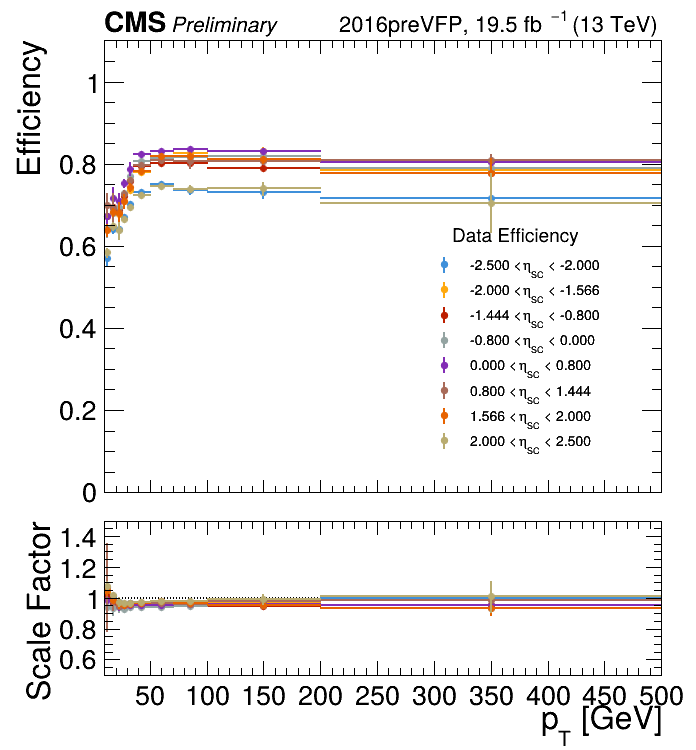
\includegraphics[width=0.45\textwidth]{Figures/analysis/EleID_eff_2016preVFP.png}}
  \hfill
  \subfloat[2016postVFP]{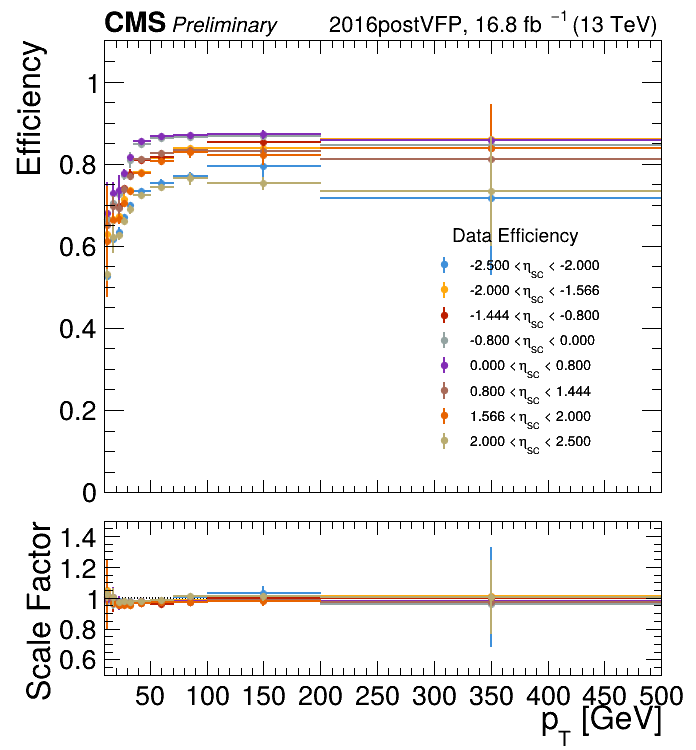
\includegraphics[width=0.45\textwidth]{Figures/analysis/EleID_eff_2016postVFP.png}} \\
  \subfloat[2017]{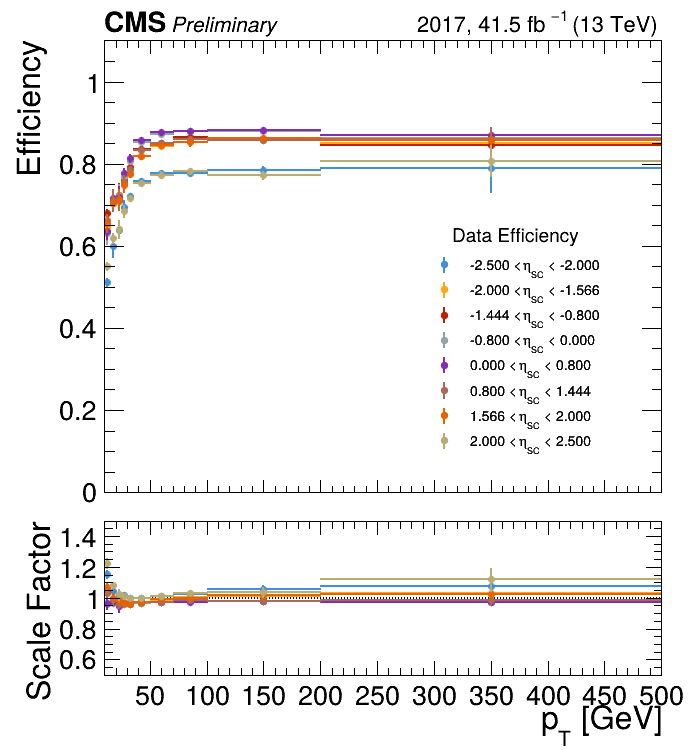
\includegraphics[width=0.45\textwidth]{Figures/analysis/EleID_eff_2017.png}}
  \hfill
  \subfloat[2018]{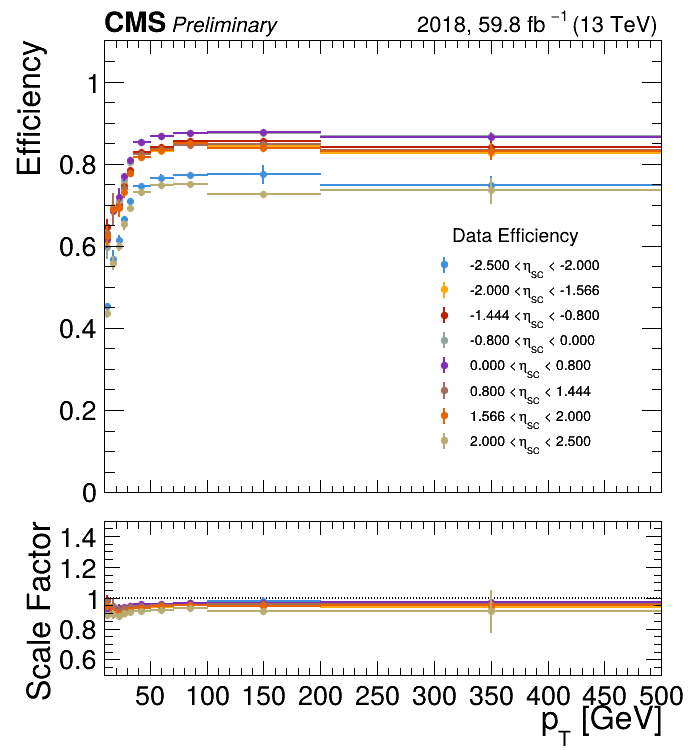
\includegraphics[width=0.45\textwidth]{Figures/analysis/EleID_eff_2018.png}}
  \caption{Electron identification efficiency as a function of $\pT$ in bins of $\eta_\text{SC}$ for the Run~2 data-taking periods. The upper panels show the data efficiency and the lower panels show the data-to-simulation scale factor.}
  \label{fig:eleid_eff_run2}
\end{figure}

\begin{figure}[htbp]
  \centering
  \subfloat[2022]{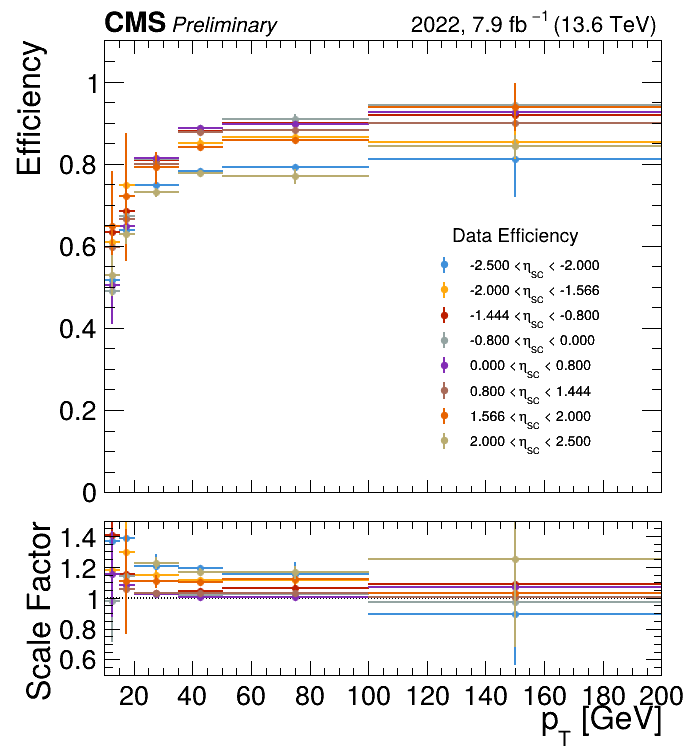
\includegraphics[width=0.45\textwidth]{Figures/analysis/EleID_eff_2022.png}}
  \hfill
  \subfloat[2022EE]{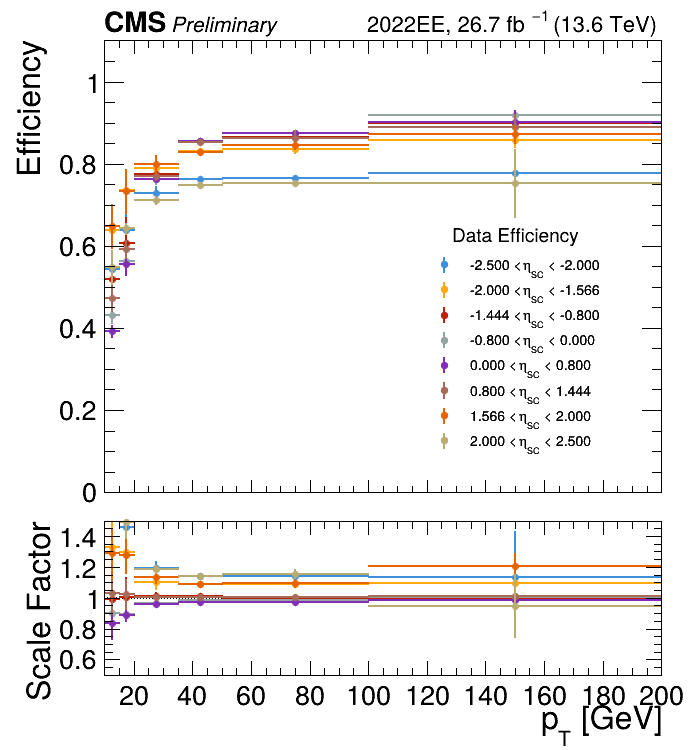
\includegraphics[width=0.45\textwidth]{Figures/analysis/EleID_eff_2022EE.png}} \\
  \subfloat[2023]{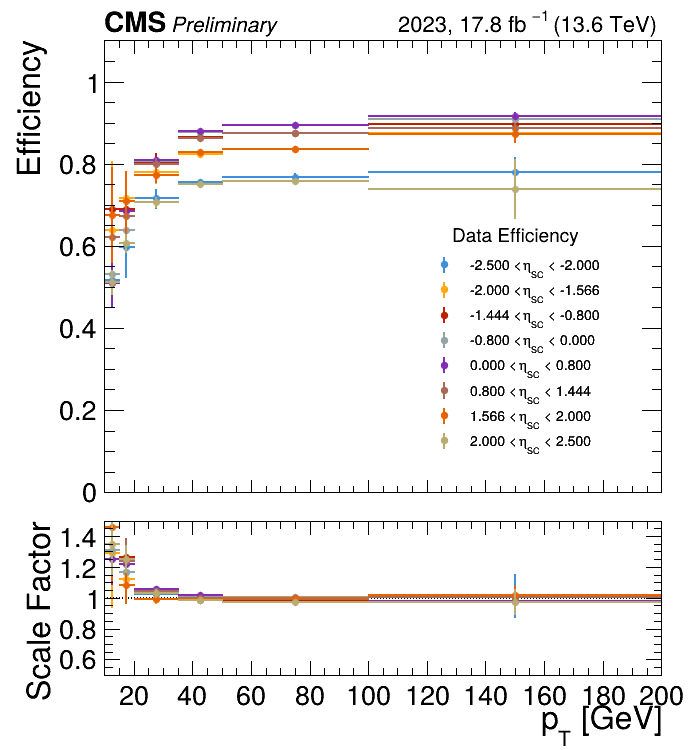
\includegraphics[width=0.45\textwidth]{Figures/analysis/EleID_eff_2023.png}}
  \hfill
  \subfloat[2023BPix]{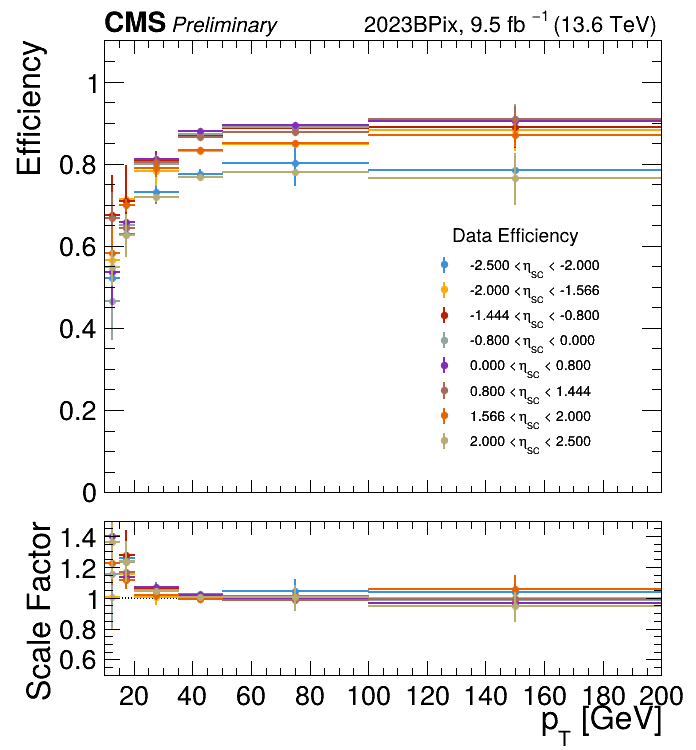
\includegraphics[width=0.45\textwidth]{Figures/analysis/EleID_eff_2023BPix.png}}
  \caption{Electron identification efficiency as a function of $\pT$ in bins of $\eta_\text{SC}$ for the Run~3 data-taking periods. The upper panels show the data efficiency and the lower panels show the data-to-simulation scale factor.}
  \label{fig:eleid_eff_run3}
\end{figure}

\begin{figure}[htbp]
  \centering
  \subfloat[2016preVFP]{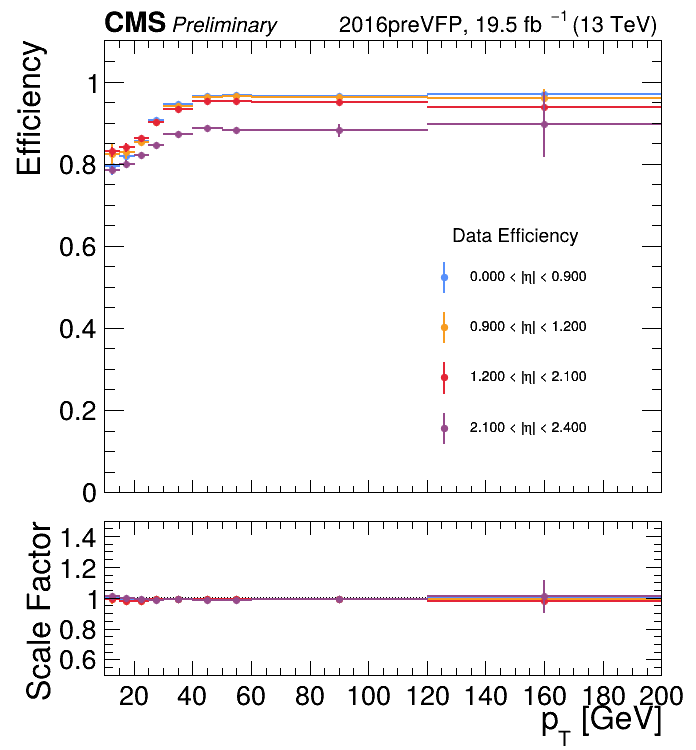
\includegraphics[width=0.45\textwidth]{Figures/analysis/MuID_eff_2016preVFP.png}}
  \hfill
  \subfloat[2016postVFP]{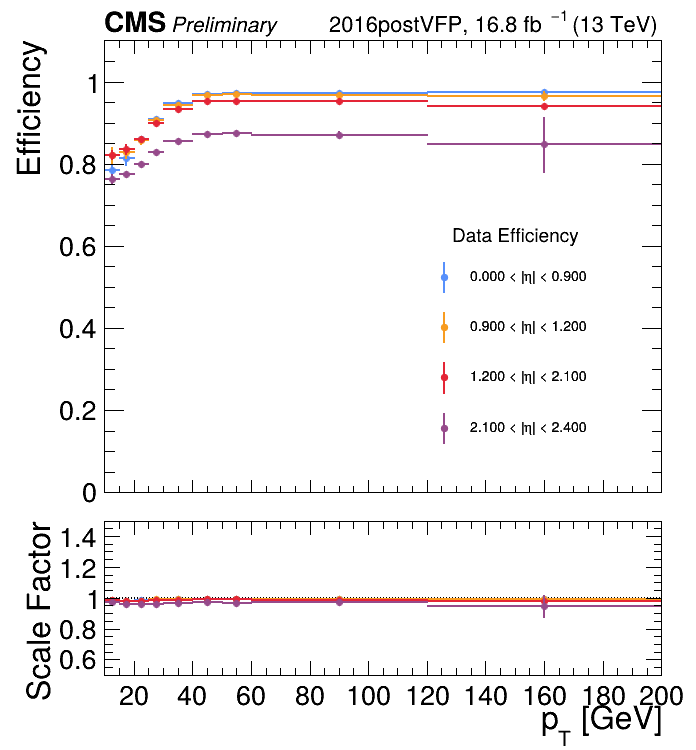
\includegraphics[width=0.45\textwidth]{Figures/analysis/MuID_eff_2016postVFP.png}} \\
  \subfloat[2017]{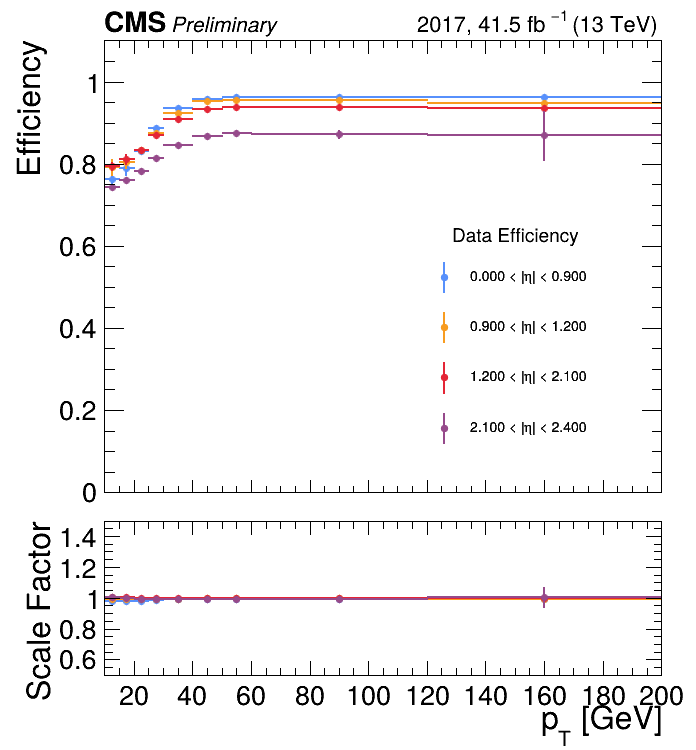
\includegraphics[width=0.45\textwidth]{Figures/analysis/MuID_eff_2017.png}}
  \hfill
  \subfloat[2018]{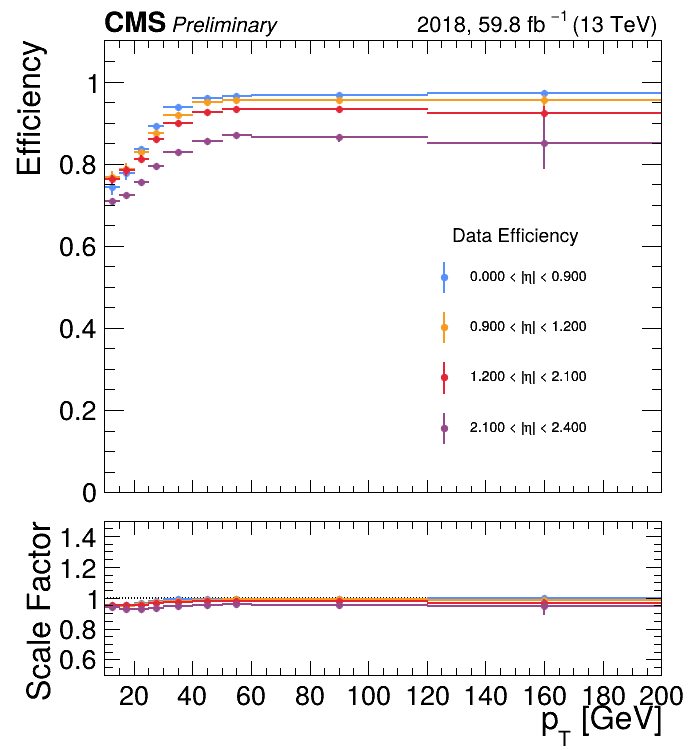
\includegraphics[width=0.45\textwidth]{Figures/analysis/MuID_eff_2018.png}}
  \caption{Muon identification efficiency as a function of $\pT$ in bins of $\eta$ for the Run~2 data-taking periods. The upper panels show the data efficiency and the lower panels show the data-to-simulation scale factor.}
  \label{fig:muid_eff_run2}
\end{figure}

\begin{figure}[htbp]
  \centering
  \subfloat[2022]{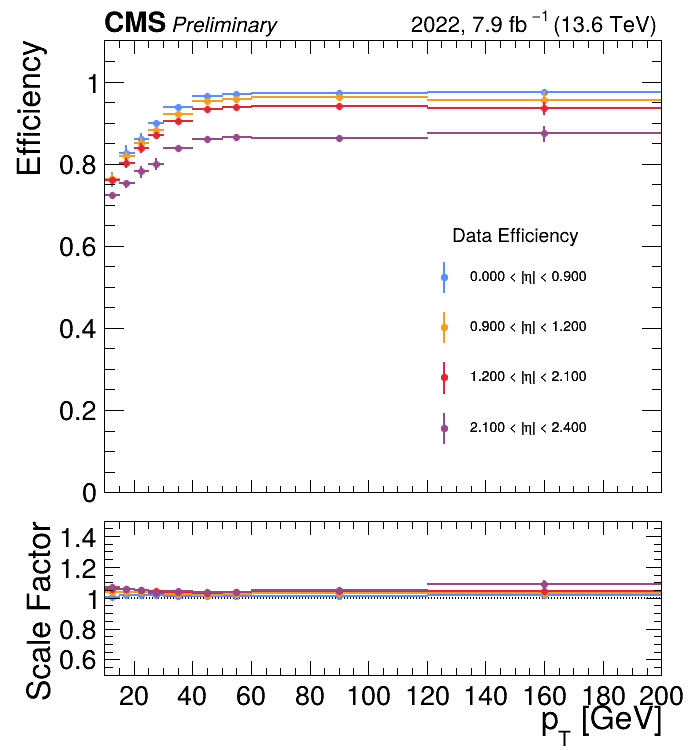
\includegraphics[width=0.45\textwidth]{Figures/analysis/MuID_eff_2022.png}}
  \hfill
  \subfloat[2022EE]{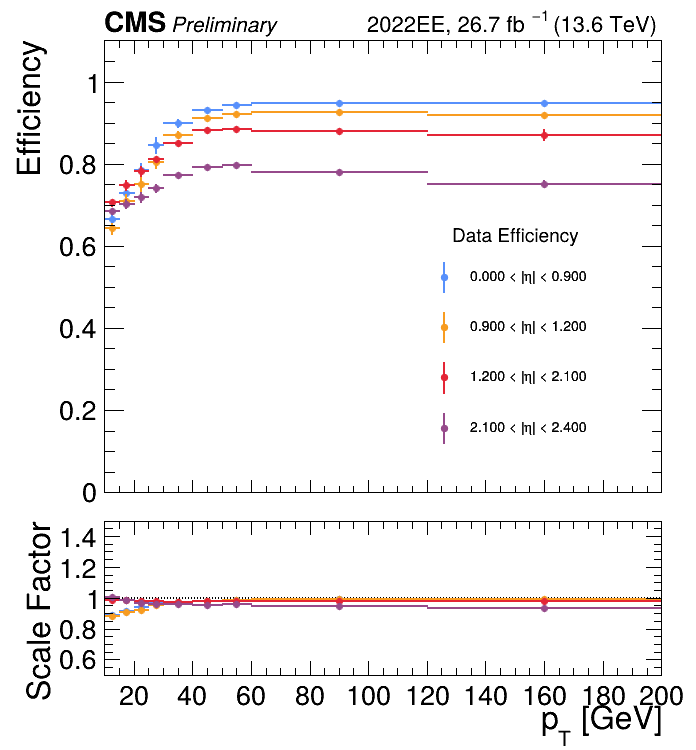
\includegraphics[width=0.45\textwidth]{Figures/analysis/MuID_eff_2022EE.png}} \\
  \subfloat[2023]{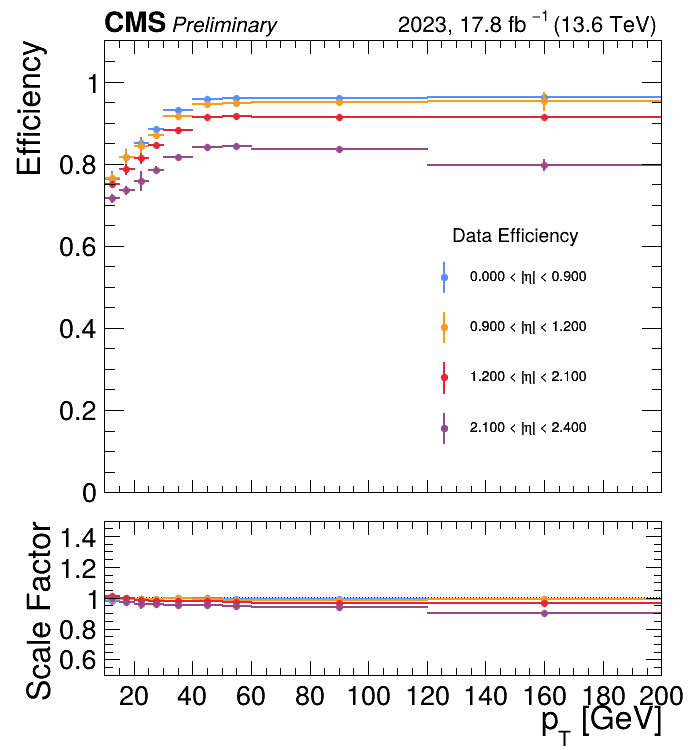
\includegraphics[width=0.45\textwidth]{Figures/analysis/MuID_eff_2023.png}}
  \hfill
  \subfloat[2023BPix]{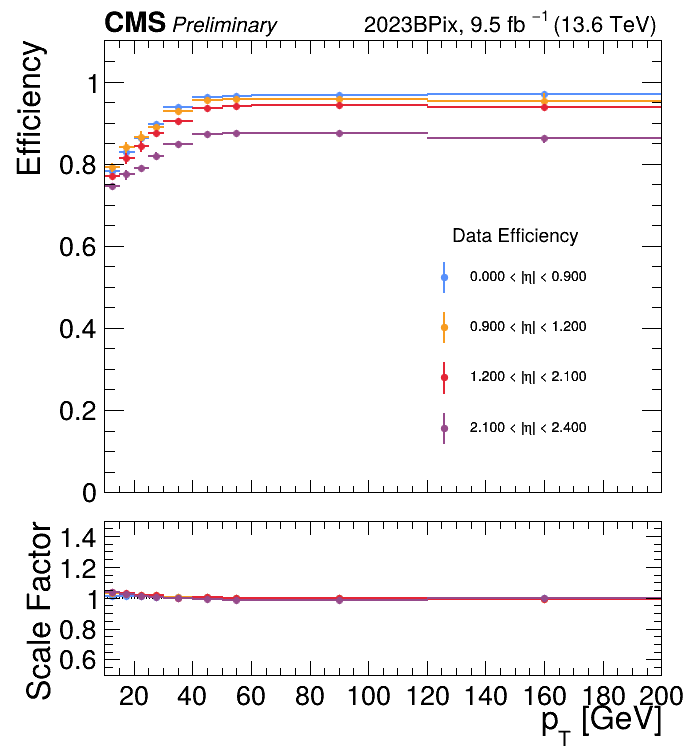
\includegraphics[width=0.45\textwidth]{Figures/analysis/MuID_eff_2023BPix.png}}
  \caption{Muon identification efficiency as a function of $\pT$ in bins of $\eta$ for the Run~3 data-taking periods. The upper panels show the data efficiency and the lower panels show the data-to-simulation scale factor.}
  \label{fig:muid_eff_run3}
\end{figure}

\subsubsection*{Trigger efficiency}

The dilepton trigger efficiency is factorized into per-lepton leg efficiencies and a pairwise filter efficiency,
\begin{equation}
\label{eq:trig_dilep}
\varepsilon(\ell_1, \ell_2) = \varepsilon_\text{leg1}(\ell_1) \times \varepsilon_\text{leg2}(\ell_2) \times \varepsilon_\text{pair}\,,
\end{equation}
where $\varepsilon_\text{leg1}$ and $\varepsilon_\text{leg2}$ denote the efficiencies for the leading and subleading trigger legs, measured as functions of $\pT$ and $\eta$ using the tag-and-probe method, and $\varepsilon_\text{pair}$ accounts for the pairwise vertex-compatibility filter applied in several trigger paths. The pairwise filter efficiency is measured using a reference trigger method and is found to be consistent with unity at the sub-percent level for all eras.

For three-lepton events, the trigger efficiency accounts for the combinatorial possibility that any qualifying lepton pair may fire the trigger. In the $\Pgm\Pgm\Pgm$ channel using dimuon triggers, the efficiency for an event with three muons ordered by $\pT$ ($\mu_1, \mu_2, \mu_3$) is
\begin{align}
\label{eq:trig_3mu}
\varepsilon(\mu_1, \mu_2, \mu_3) &= \varepsilon_\text{leg1}(\mu_1) \left[ \varepsilon_\text{leg2}(\mu_2)\,\varepsilon_\text{pair} + \left(1 - \varepsilon_\text{leg2}(\mu_2)\right) \varepsilon_\text{leg2}(\mu_3)\,\varepsilon_\text{pair} \right] \nonumber \\
&\quad + \left(1 - \varepsilon_\text{leg1}(\mu_1)\right) \varepsilon_\text{leg1}(\mu_2)\,\varepsilon_\text{leg2}(\mu_3)\,\varepsilon_\text{pair}\,.
\end{align}
In the $\Pe\Pgm\Pgm$ channel using electron-muon cross-triggers, the efficiency for an event with one electron and two muons is
\begin{equation}
\label{eq:trig_emu}
\varepsilon(e, \mu_1, \mu_2) = \varepsilon_e(e) \left[ \varepsilon_\mu(\mu_1)\,\varepsilon_\text{pair} + \left(1 - \varepsilon_\mu(\mu_1)\right) \varepsilon_\mu(\mu_2)\,\varepsilon_\text{pair} \right] .
\end{equation}
The trigger scale factor for each event is computed as the ratio of the data and MC efficiencies,
\begin{equation}
\text{SF}_\text{trig} = \frac{\varepsilon_\text{data}}{\varepsilon_\text{MC}}\,.
\end{equation}

The measured per-leg trigger efficiencies are grouped by trigger path in Figs.~\ref{fig:trig_dblmu_run2}--\ref{fig:trig_mu8el23_run3}. For the dimuon triggers, the leading ($\pT > 17$\GeV) and subleading ($\pT > 8$\GeV) muon legs are measured separately. For the electron-muon cross-triggers, two paths are used: \texttt{Mu23\_El12} (muon $\pT > 23$\GeV, electron $\pT > 12$\GeV) and \texttt{Mu8\_El23} (muon $\pT > 8$\GeV, electron $\pT > 23$\GeV).

\begin{sidewaysfigure}[p]
  \centering
  \subfloat[2016preVFP]{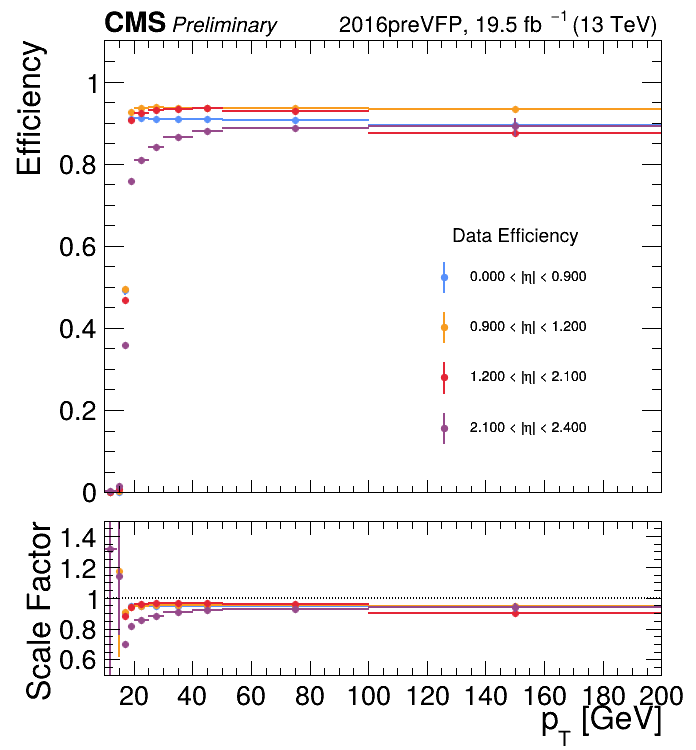
\includegraphics[width=0.23\textwidth]{Figures/analysis/DblMu_MU17Leg_eff_2016preVFP.png}}
  \hfill
  \subfloat[2016postVFP]{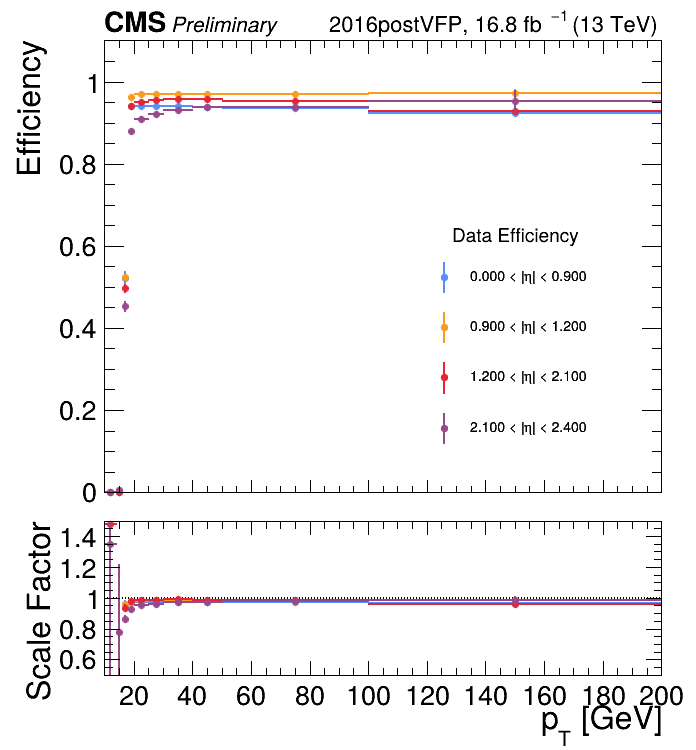
\includegraphics[width=0.23\textwidth]{Figures/analysis/DblMu_MU17Leg_eff_2016postVFP.png}}
  \hfill
  \subfloat[2017]{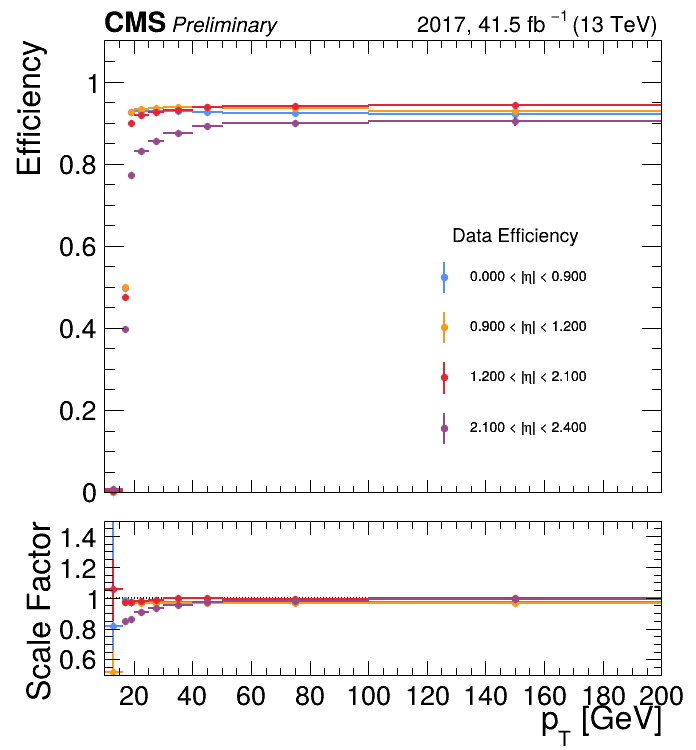
\includegraphics[width=0.23\textwidth]{Figures/analysis/DblMu_MU17Leg_eff_2017.png}}
  \hfill
  \subfloat[2018]{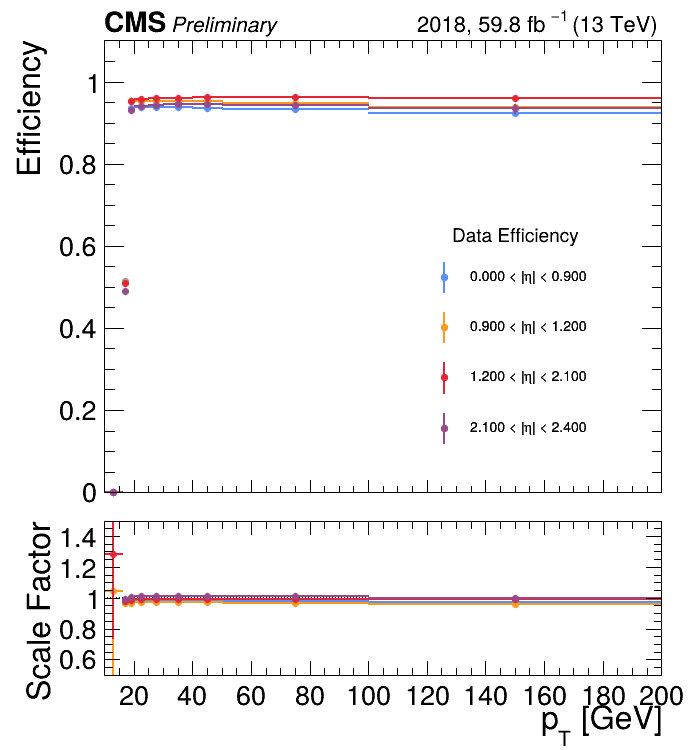
\includegraphics[width=0.23\textwidth]{Figures/analysis/DblMu_MU17Leg_eff_2018.png}}
  \\
  \subfloat[2016preVFP]{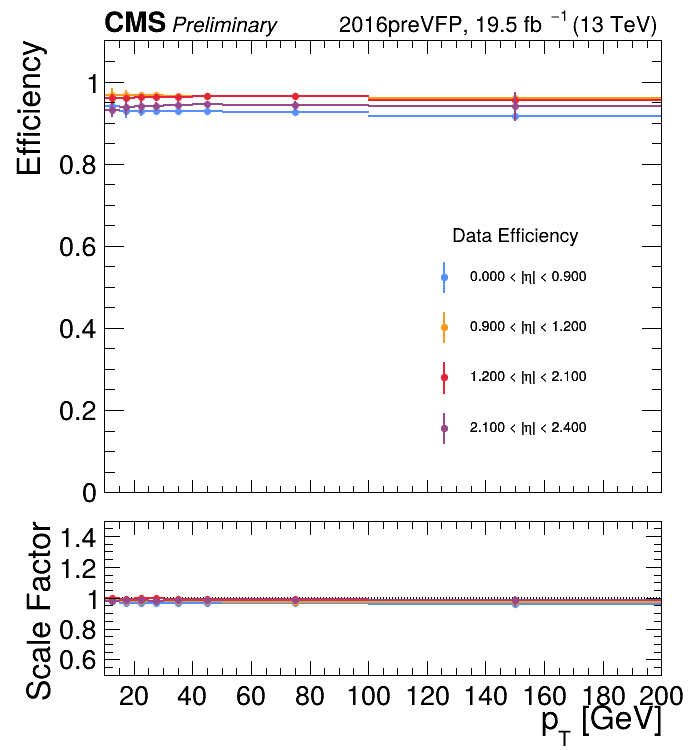
\includegraphics[width=0.23\textwidth]{Figures/analysis/DblMu_MU8Leg_eff_2016preVFP.png}}
  \hfill
  \subfloat[2016postVFP]{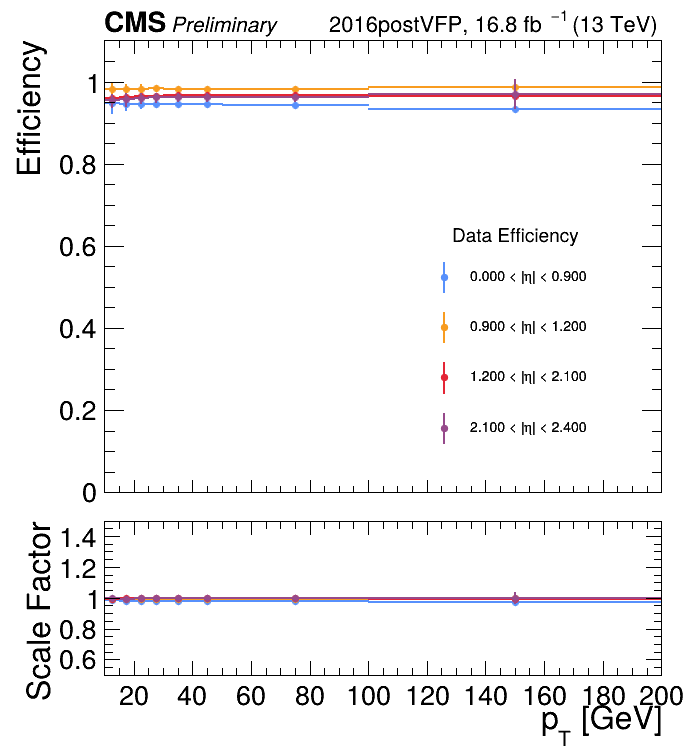
\includegraphics[width=0.23\textwidth]{Figures/analysis/DblMu_MU8Leg_eff_2016postVFP.png}}
  \hfill
  \subfloat[2017]{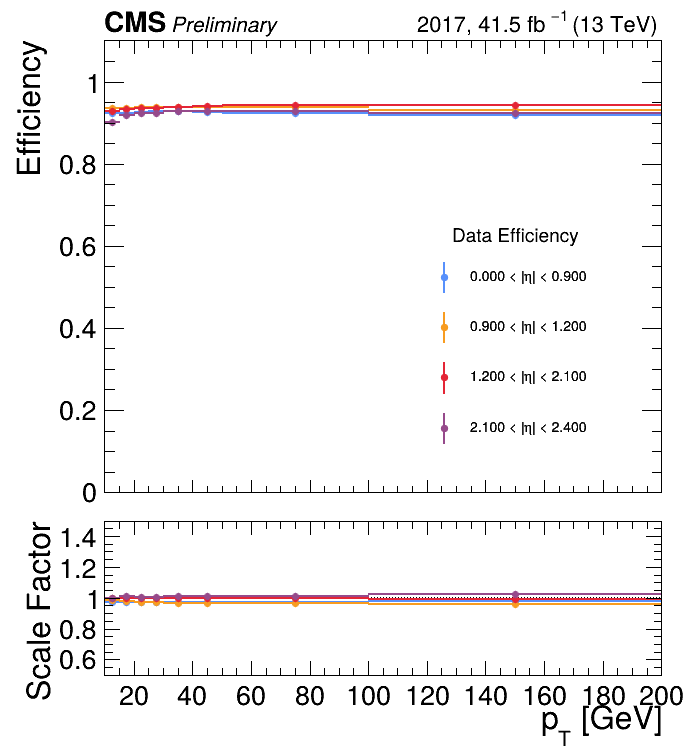
\includegraphics[width=0.23\textwidth]{Figures/analysis/DblMu_MU8Leg_eff_2017.png}}
  \hfill
  \subfloat[2018]{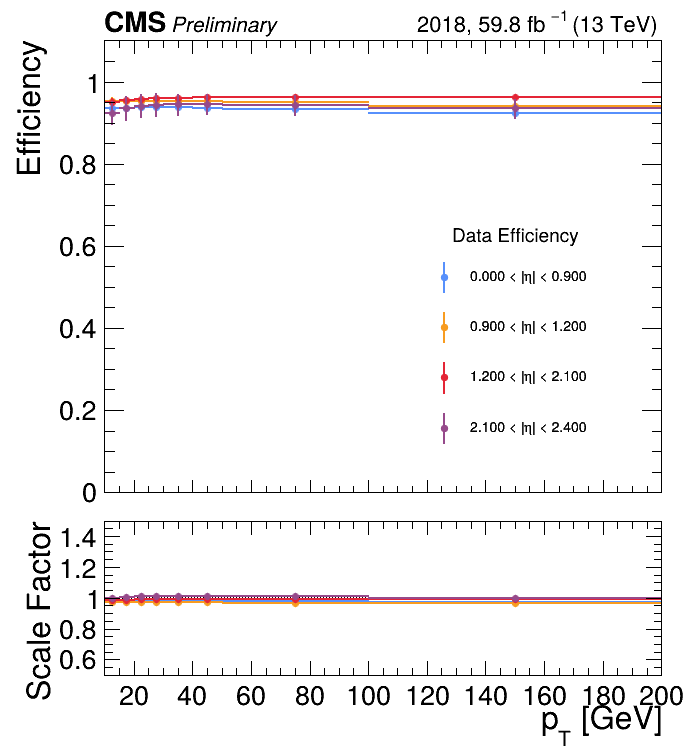
\includegraphics[width=0.23\textwidth]{Figures/analysis/DblMu_MU8Leg_eff_2018.png}}
  \caption{Dimuon trigger leg efficiencies as functions of muon $\pT$ in bins of $\eta$ for the Run~2 data-taking periods. The upper row shows the leading leg ($\pT > 17$\GeV), and the lower row shows the subleading leg ($\pT > 8$\GeV).}
  \label{fig:trig_dblmu_run2}
\end{sidewaysfigure}

\begin{sidewaysfigure}[p]
  \centering
  \subfloat[2022]{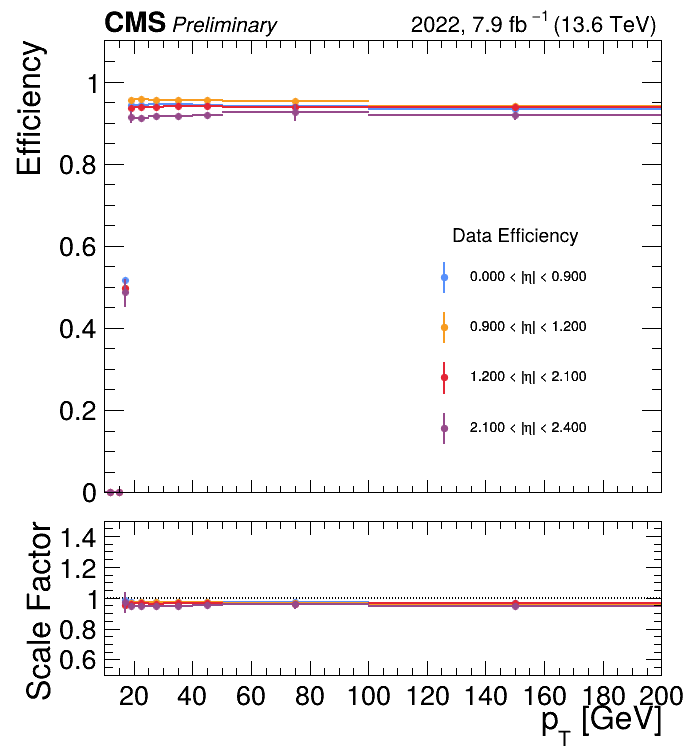
\includegraphics[width=0.23\textwidth]{Figures/analysis/DblMu_MU17Leg_eff_2022.png}}
  \hfill
  \subfloat[2022EE]{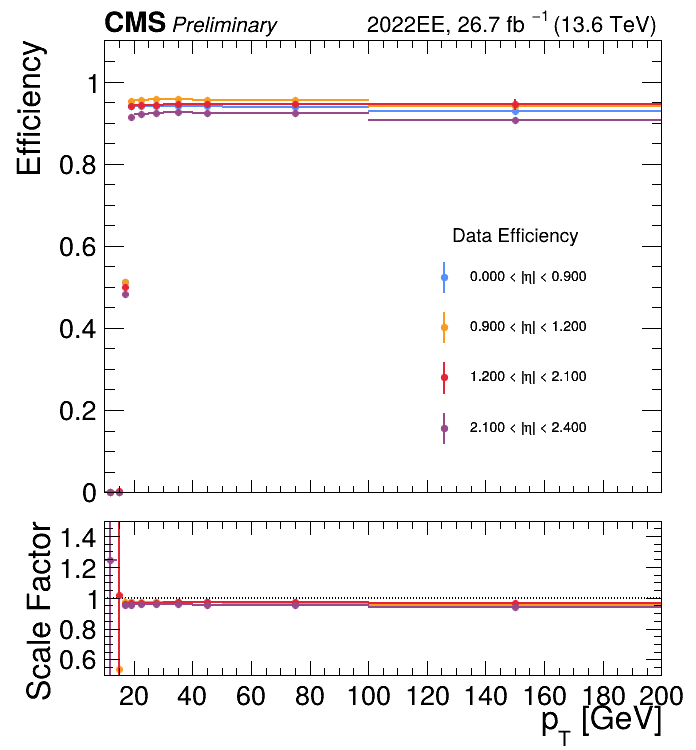
\includegraphics[width=0.23\textwidth]{Figures/analysis/DblMu_MU17Leg_eff_2022EE.png}}
  \hfill
  \subfloat[2023]{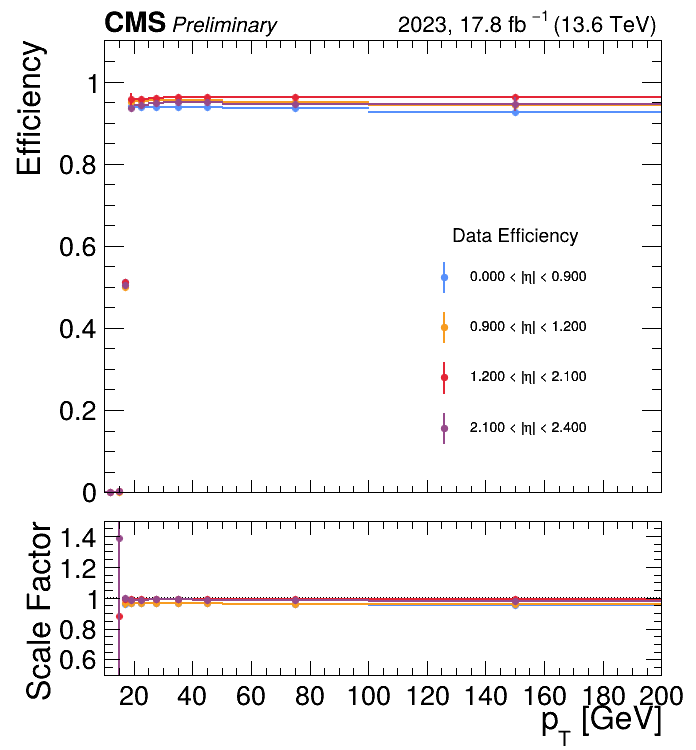
\includegraphics[width=0.23\textwidth]{Figures/analysis/DblMu_MU17Leg_eff_2023.png}}
  \hfill
  \subfloat[2023BPix]{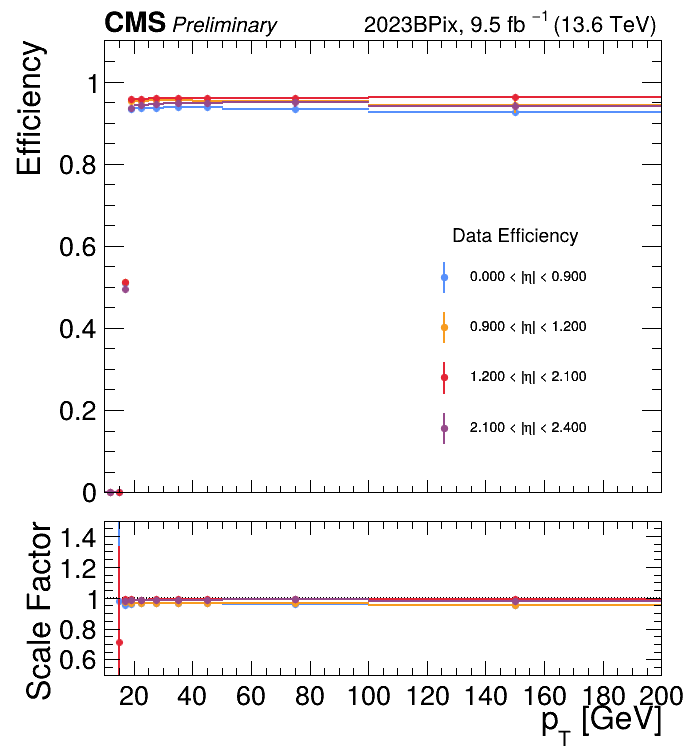
\includegraphics[width=0.23\textwidth]{Figures/analysis/DblMu_MU17Leg_eff_2023BPix.png}}
  \\
  \subfloat[2022]{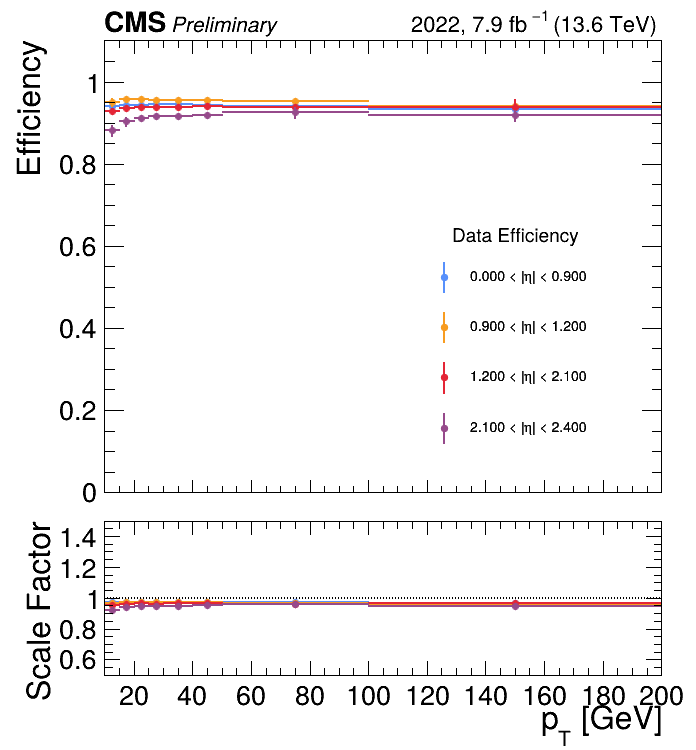
\includegraphics[width=0.23\textwidth]{Figures/analysis/DblMu_MU8Leg_eff_2022.png}}
  \hfill
  \subfloat[2022EE]{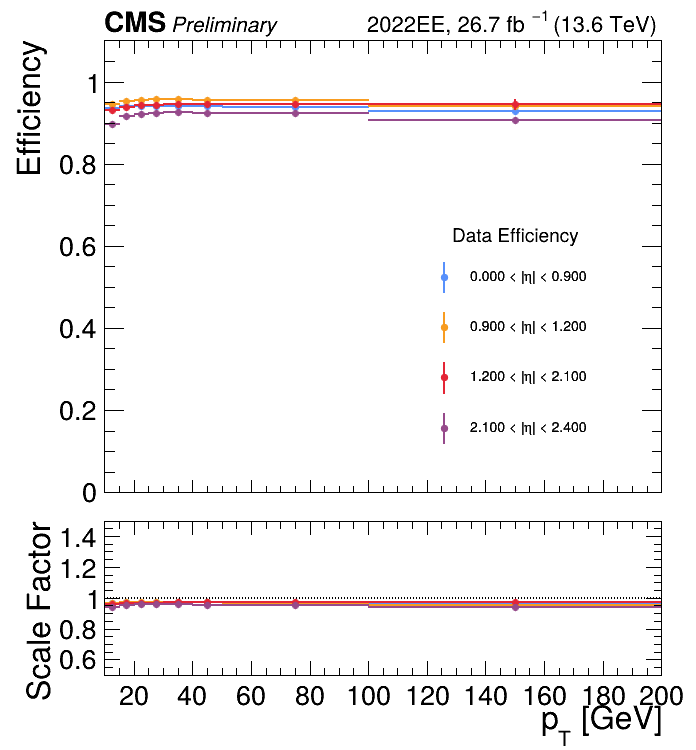
\includegraphics[width=0.23\textwidth]{Figures/analysis/DblMu_MU8Leg_eff_2022EE.png}}
  \hfill
  \subfloat[2023]{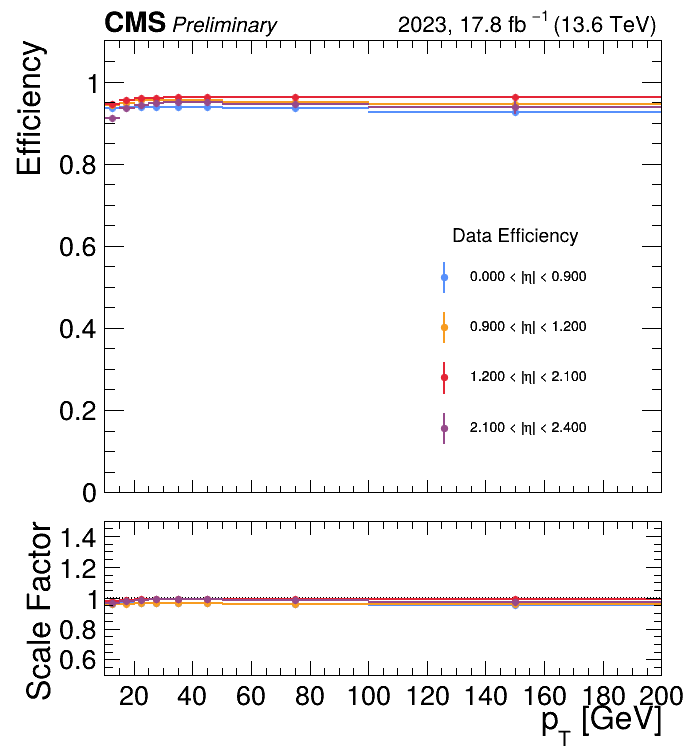
\includegraphics[width=0.23\textwidth]{Figures/analysis/DblMu_MU8Leg_eff_2023.png}}
  \hfill
  \subfloat[2023BPix]{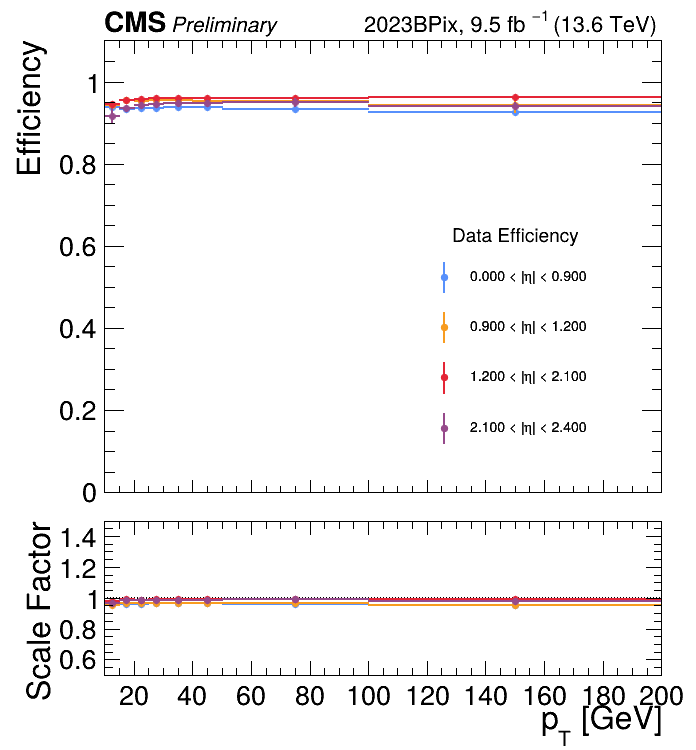
\includegraphics[width=0.23\textwidth]{Figures/analysis/DblMu_MU8Leg_eff_2023BPix.png}}
  \caption{Dimuon trigger leg efficiencies as functions of muon $\pT$ in bins of $\eta$ for the Run~3 data-taking periods. The upper row shows the leading leg ($\pT > 17$\GeV), and the lower row shows the subleading leg ($\pT > 8$\GeV).}
  \label{fig:trig_dblmu_run3}
\end{sidewaysfigure}

\begin{sidewaysfigure}[p]
  \centering
  \subfloat[2016preVFP]{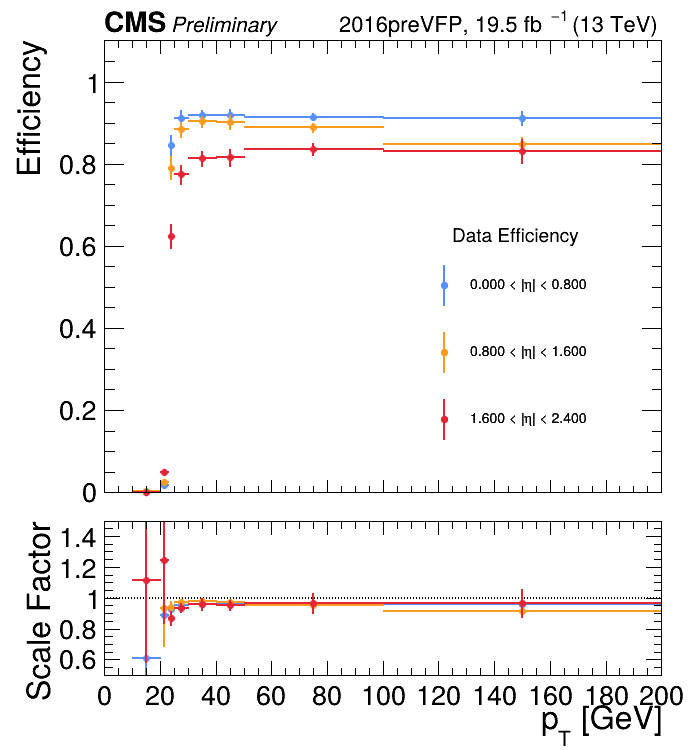
\includegraphics[width=0.23\textwidth]{Figures/analysis/Mu23El12_muon_eff_2016preVFP.png}}
  \hfill
  \subfloat[2016postVFP]{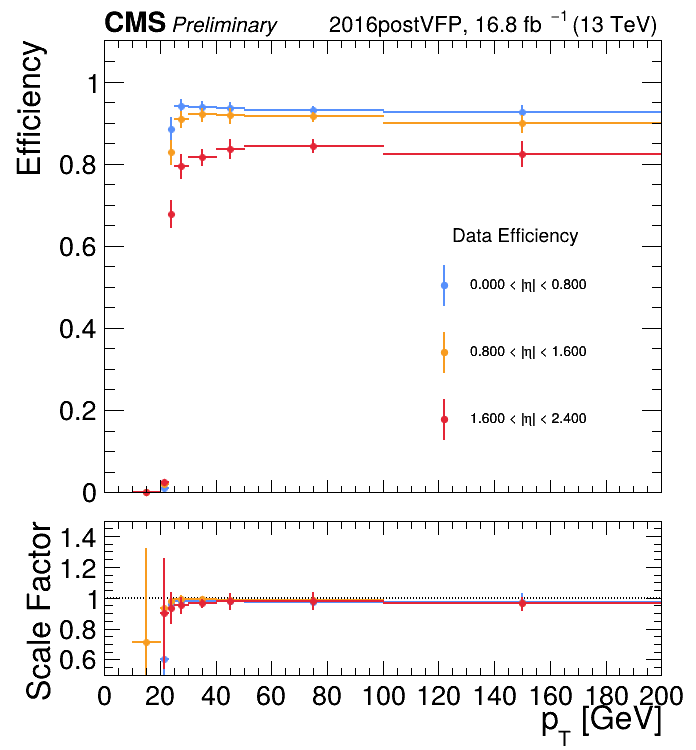
\includegraphics[width=0.23\textwidth]{Figures/analysis/Mu23El12_muon_eff_2016postVFP.png}}
  \hfill
  \subfloat[2017]{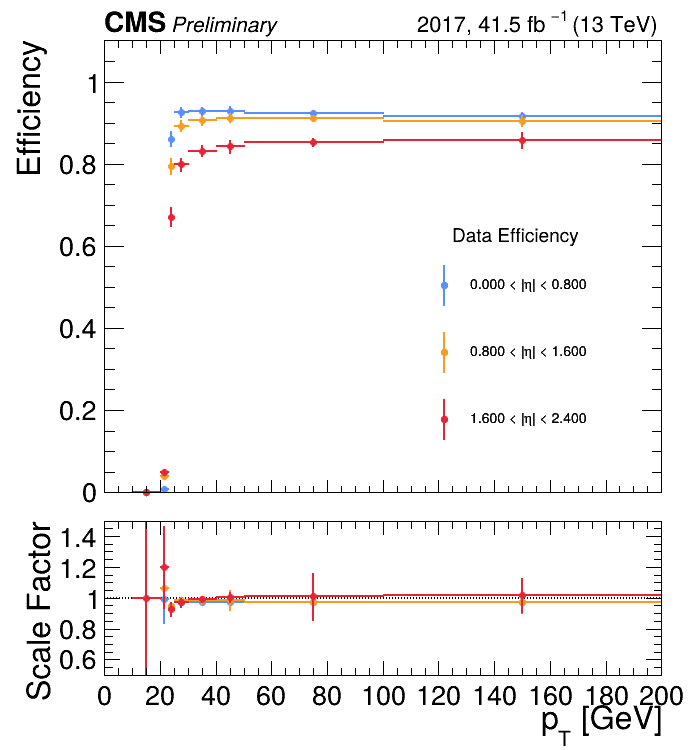
\includegraphics[width=0.23\textwidth]{Figures/analysis/Mu23El12_muon_eff_2017.png}}
  \hfill
  \subfloat[2018]{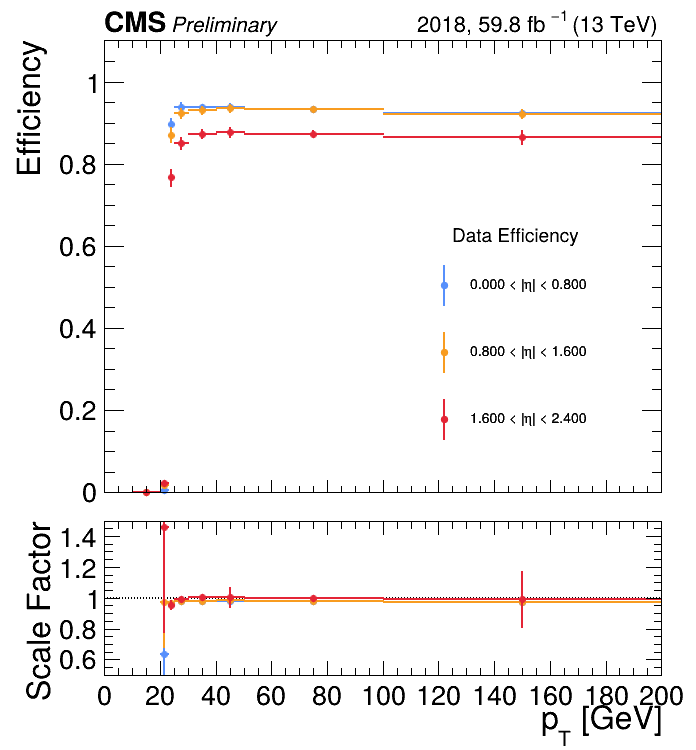
\includegraphics[width=0.23\textwidth]{Figures/analysis/Mu23El12_muon_eff_2018.png}}
  \\
  \subfloat[2016preVFP]{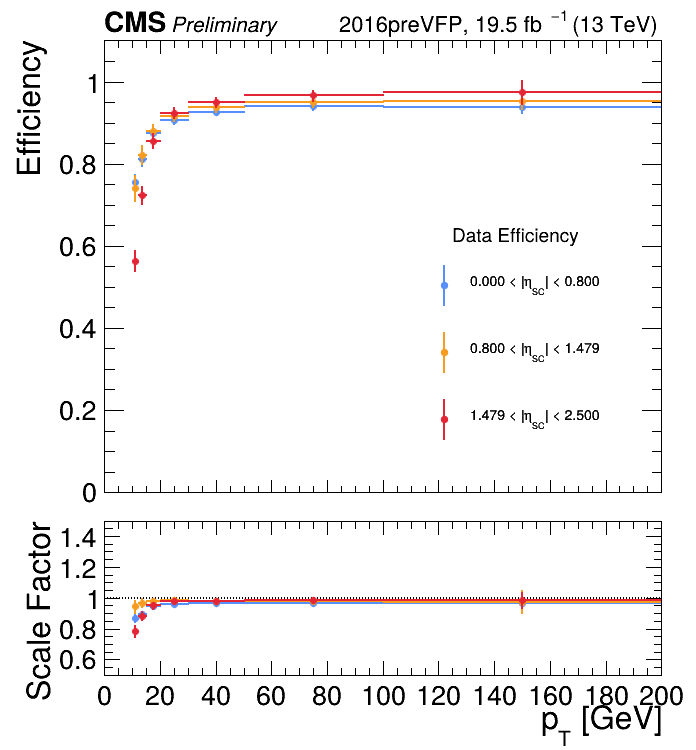
\includegraphics[width=0.23\textwidth]{Figures/analysis/Mu23El12_electron_eff_2016preVFP.png}}
  \hfill
  \subfloat[2016postVFP]{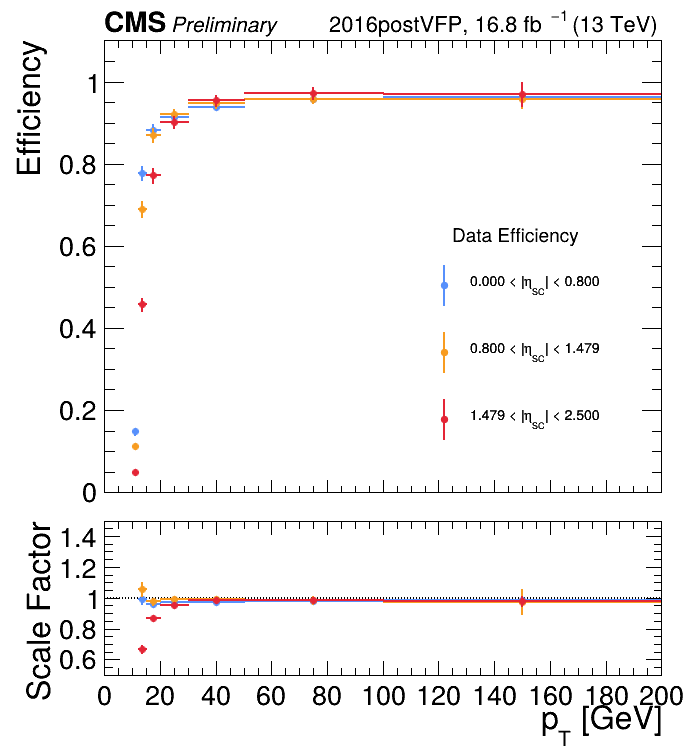
\includegraphics[width=0.23\textwidth]{Figures/analysis/Mu23El12_electron_eff_2016postVFP.png}}
  \hfill
  \subfloat[2017]{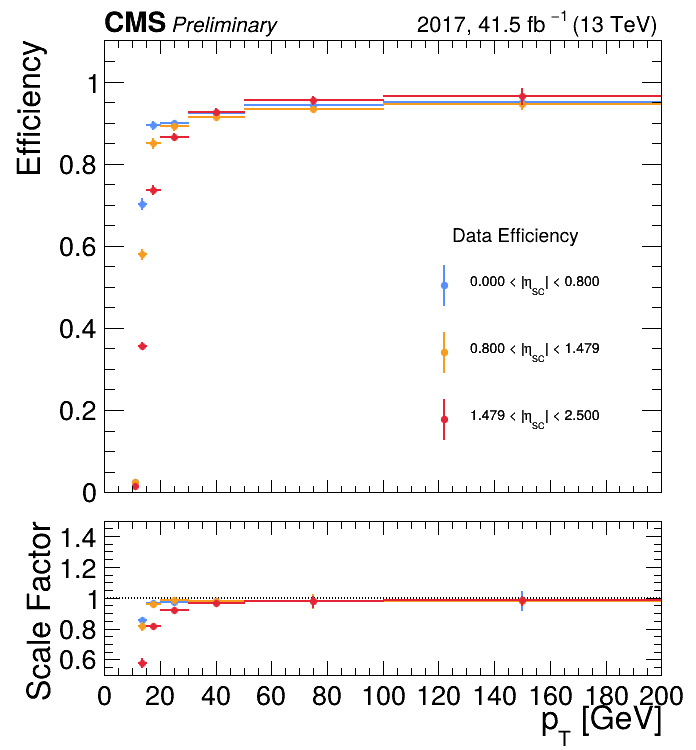
\includegraphics[width=0.23\textwidth]{Figures/analysis/Mu23El12_electron_eff_2017.png}}
  \hfill
  \subfloat[2018]{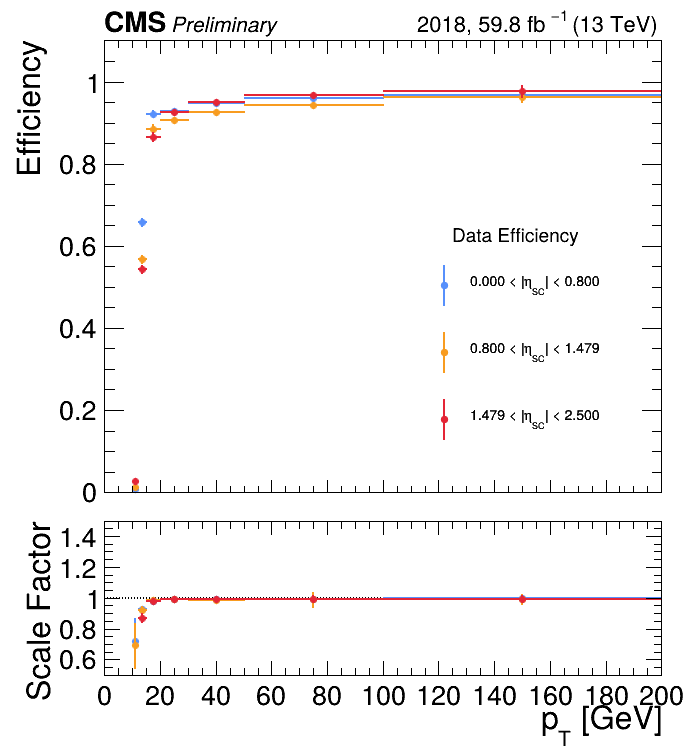
\includegraphics[width=0.23\textwidth]{Figures/analysis/Mu23El12_electron_eff_2018.png}}
  \caption{Leg efficiencies for the \texttt{Mu23\_El12} cross-trigger as functions of lepton $\pT$ in bins of $\eta$ or $\eta_\text{SC}$ for the Run~2 data-taking periods. The upper row shows the muon leg ($\pT > 23$\GeV), and the lower row shows the electron leg ($\pT > 12$\GeV).}
  \label{fig:trig_mu23el12_run2}
\end{sidewaysfigure}

\begin{sidewaysfigure}[p]
  \centering
  \subfloat[2022]{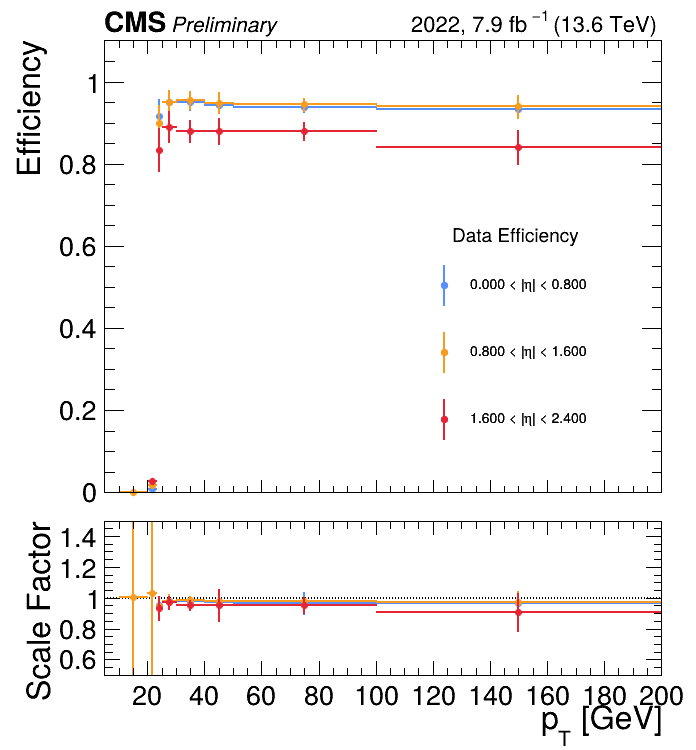
\includegraphics[width=0.21\textwidth]{Figures/analysis/Mu23El12_muon_eff_2022.png}}
  \hfill
  \subfloat[2022EE]{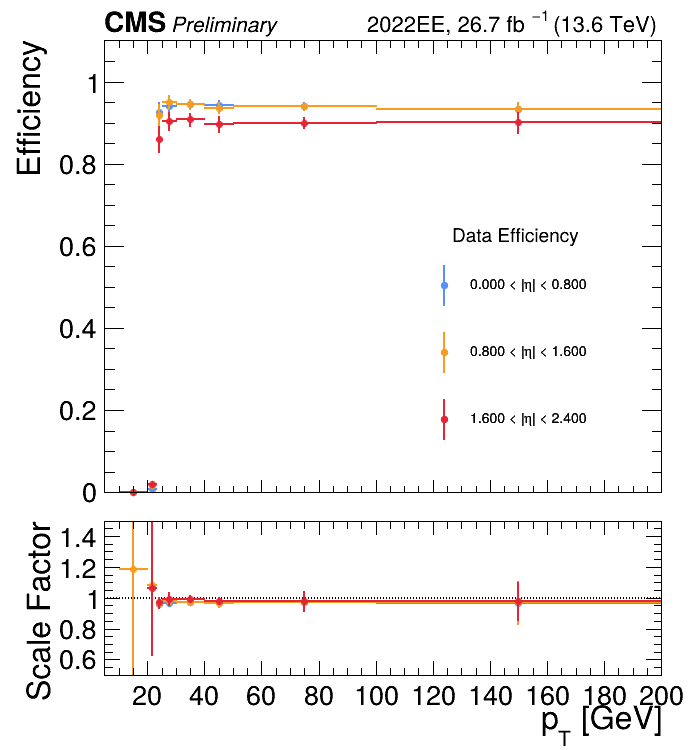
\includegraphics[width=0.21\textwidth]{Figures/analysis/Mu23El12_muon_eff_2022EE.png}}
  \hfill
  \subfloat[2023]{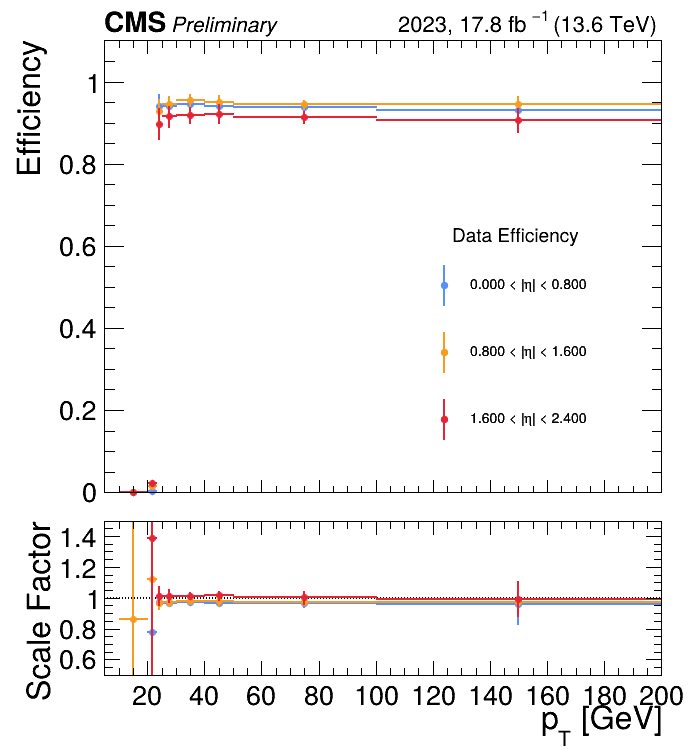
\includegraphics[width=0.21\textwidth]{Figures/analysis/Mu23El12_muon_eff_2023.png}}
  \hfill
  \subfloat[2023BPix]{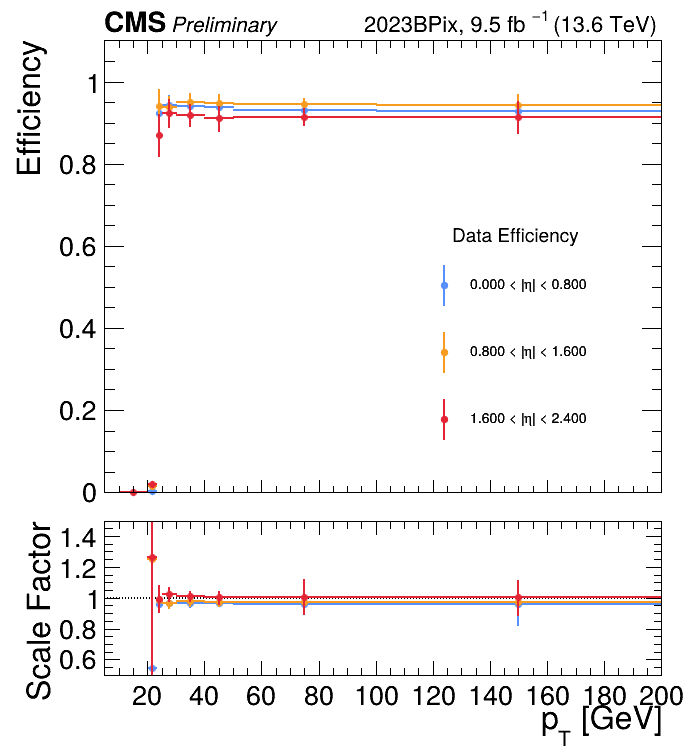
\includegraphics[width=0.21\textwidth]{Figures/analysis/Mu23El12_muon_eff_2023BPix.png}}
  \\
  \subfloat[2022]{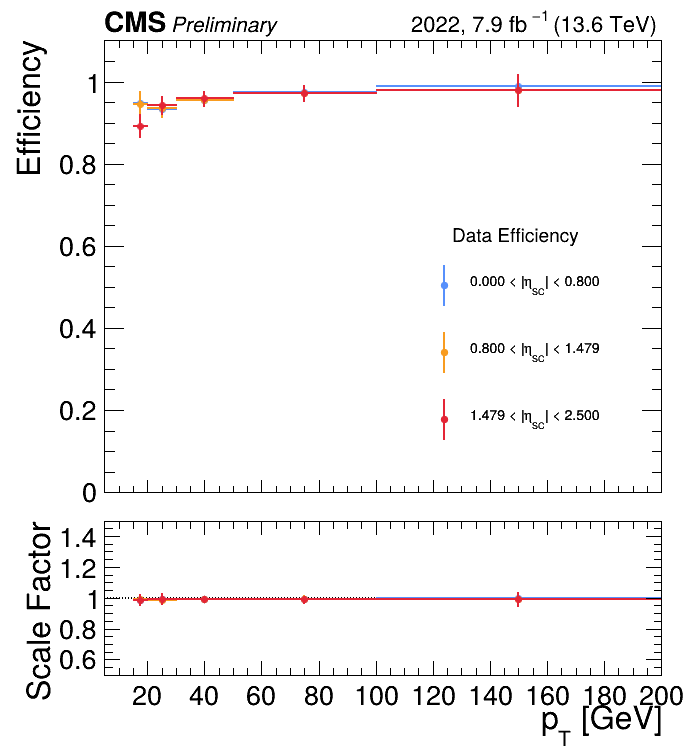
\includegraphics[width=0.21\textwidth]{Figures/analysis/Mu23El12_electron_eff_2022.png}}
  \hfill
  \subfloat[2022EE]{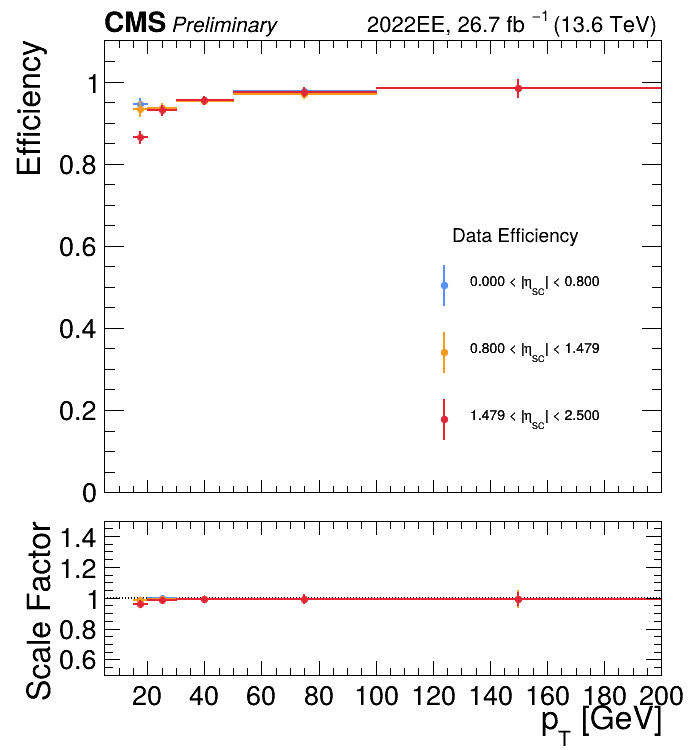
\includegraphics[width=0.21\textwidth]{Figures/analysis/Mu23El12_electron_eff_2022EE.png}}
  \hfill
  \subfloat[2023]{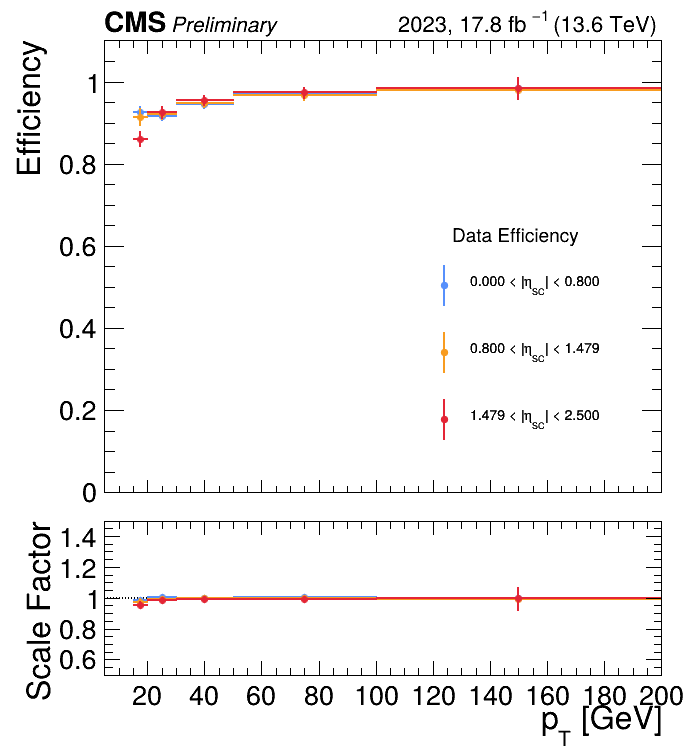
\includegraphics[width=0.21\textwidth]{Figures/analysis/Mu23El12_electron_eff_2023.png}}
  \hfill
  \subfloat[2023BPix]{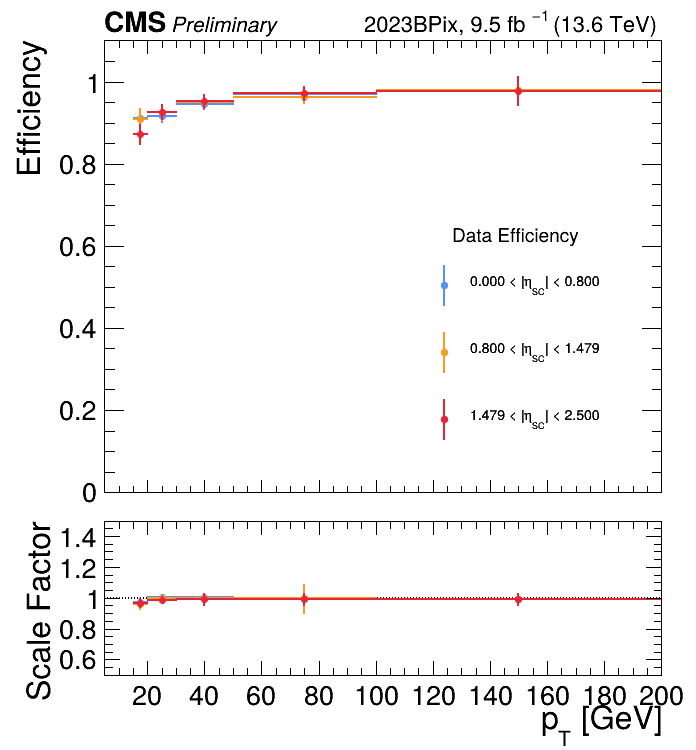
\includegraphics[width=0.21\textwidth]{Figures/analysis/Mu23El12_electron_eff_2023BPix.png}}
  \caption{Leg efficiencies for the \texttt{Mu23\_El12} cross-trigger in the Run~3 data-taking periods. The upper and lower rows show the muon ($\pT > 23$\GeV) and electron ($\pT > 12$\GeV) legs, respectively.}
  \label{fig:trig_mu23el12_run3}
\end{sidewaysfigure}

\begin{sidewaysfigure}[p]
  \centering
  \subfloat[2016preVFP]{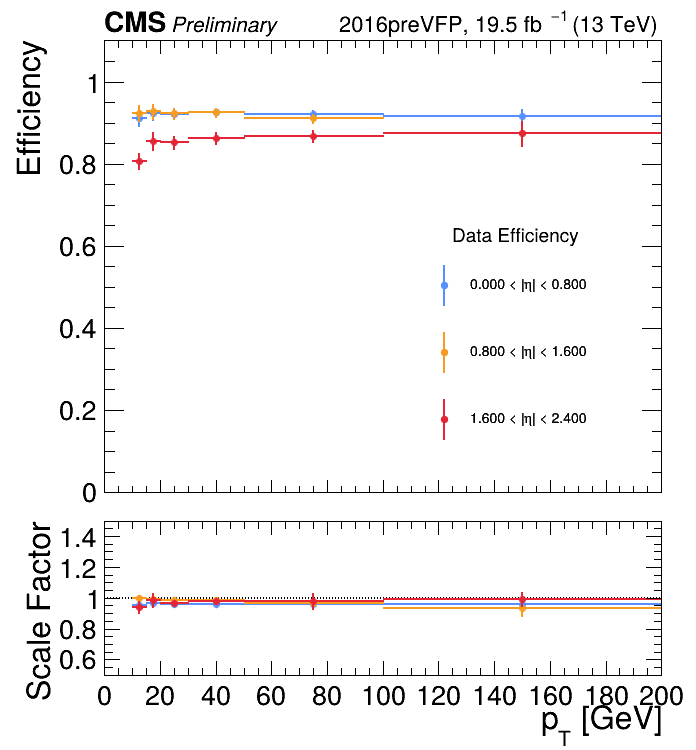
\includegraphics[width=0.23\textwidth]{Figures/analysis/Mu8El23_muon_eff_2016preVFP.png}}
  \hfill
  \subfloat[2016postVFP]{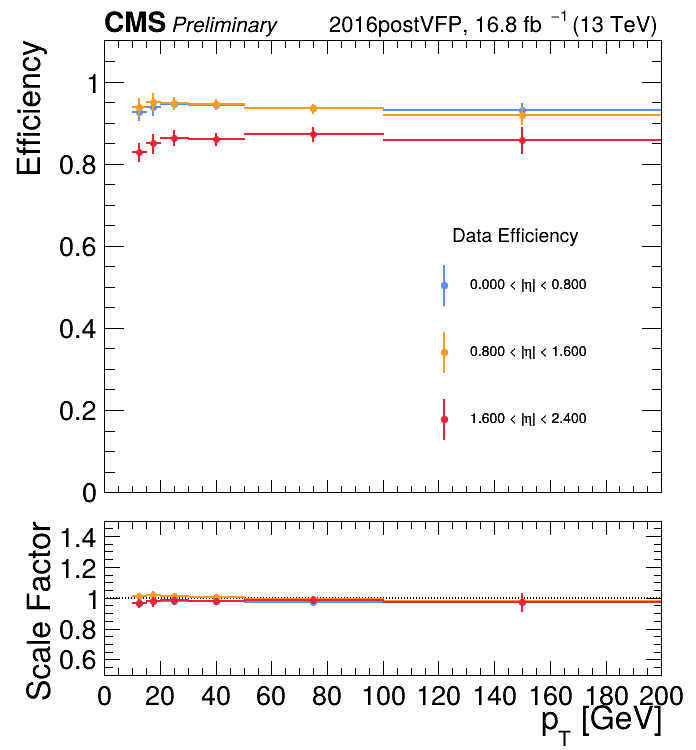
\includegraphics[width=0.23\textwidth]{Figures/analysis/Mu8El23_muon_eff_2016postVFP.png}}
  \hfill
  \subfloat[2017]{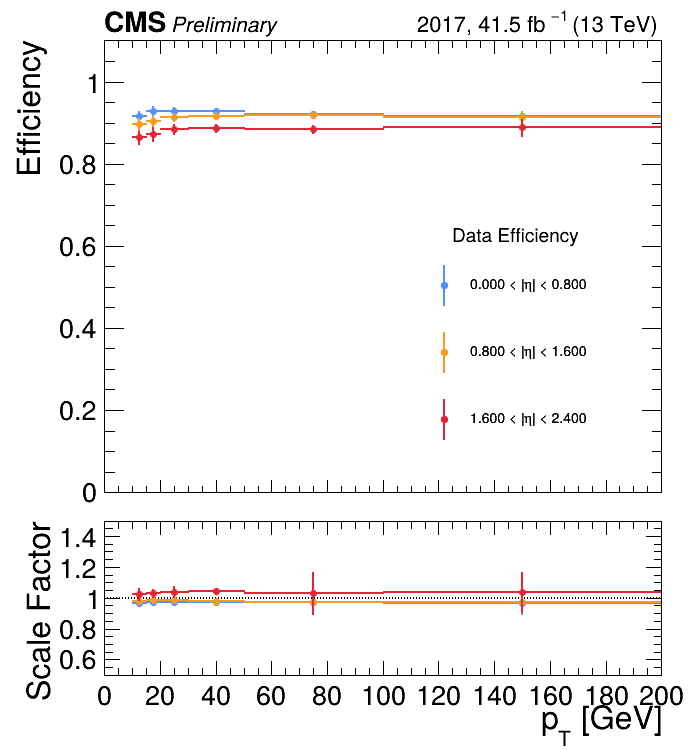
\includegraphics[width=0.23\textwidth]{Figures/analysis/Mu8El23_muon_eff_2017.png}}
  \hfill
  \subfloat[2018]{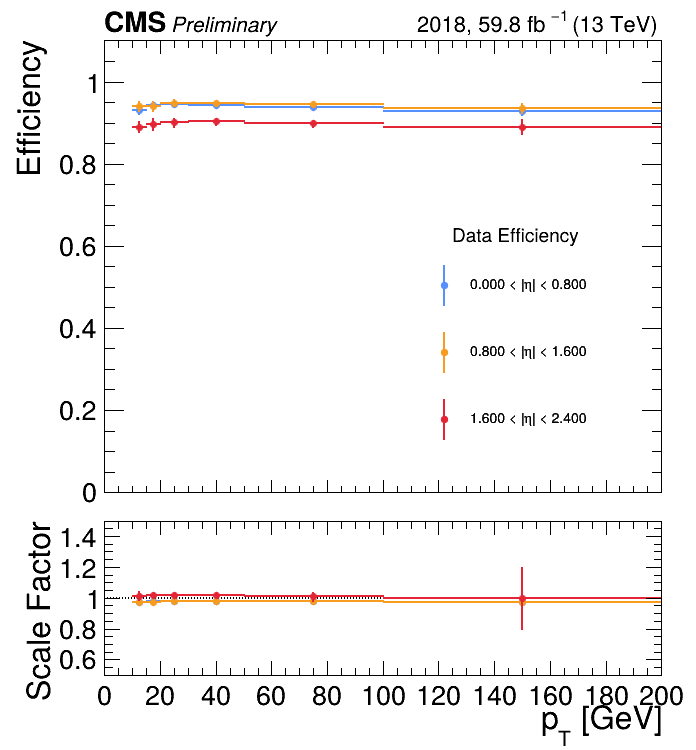
\includegraphics[width=0.23\textwidth]{Figures/analysis/Mu8El23_muon_eff_2018.png}}
  \\
  \subfloat[2016preVFP]{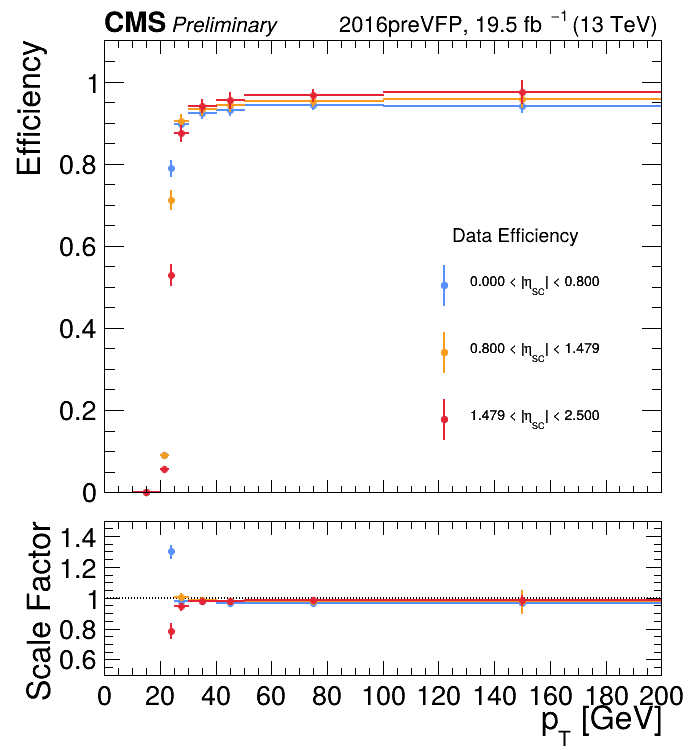
\includegraphics[width=0.23\textwidth]{Figures/analysis/Mu8El23_electron_eff_2016preVFP.png}}
  \hfill
  \subfloat[2016postVFP]{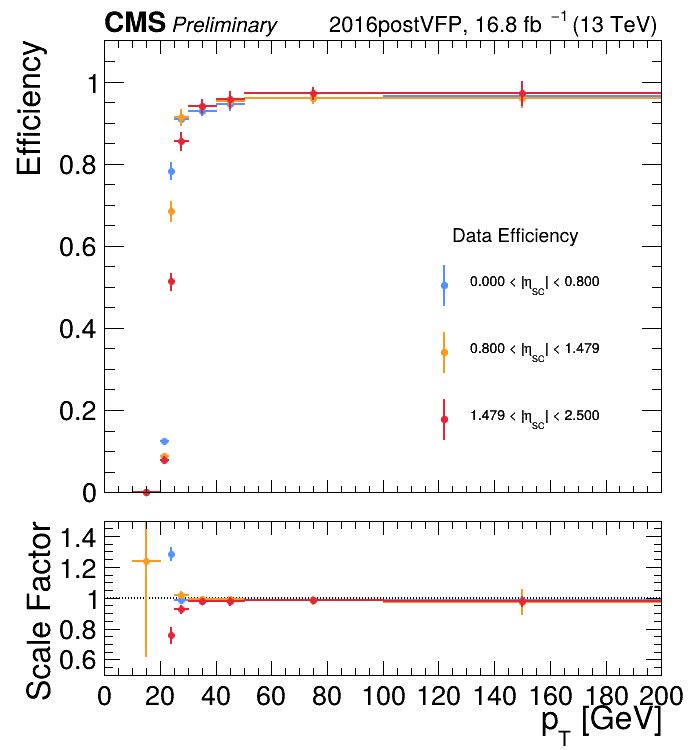
\includegraphics[width=0.23\textwidth]{Figures/analysis/Mu8El23_electron_eff_2016postVFP.png}}
  \hfill
  \subfloat[2017]{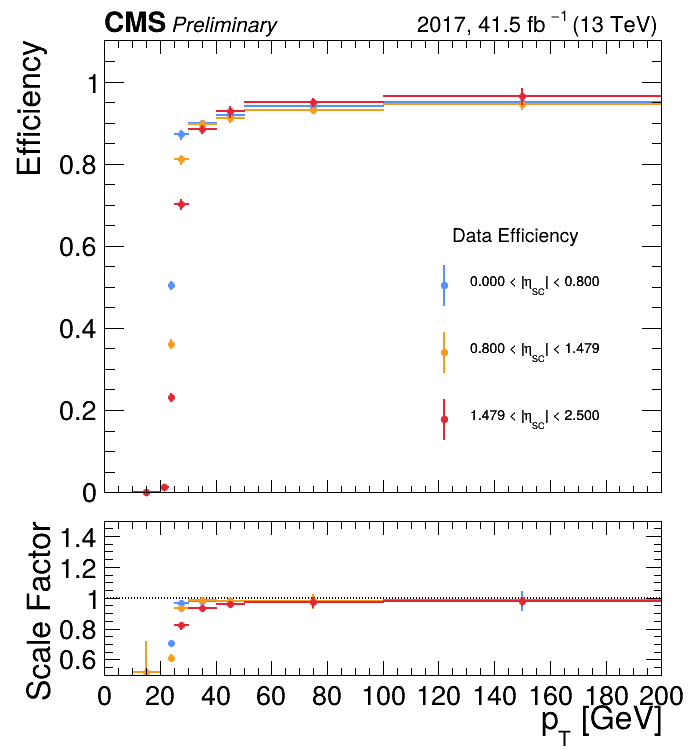
\includegraphics[width=0.23\textwidth]{Figures/analysis/Mu8El23_electron_eff_2017.png}}
  \hfill
  \subfloat[2018]{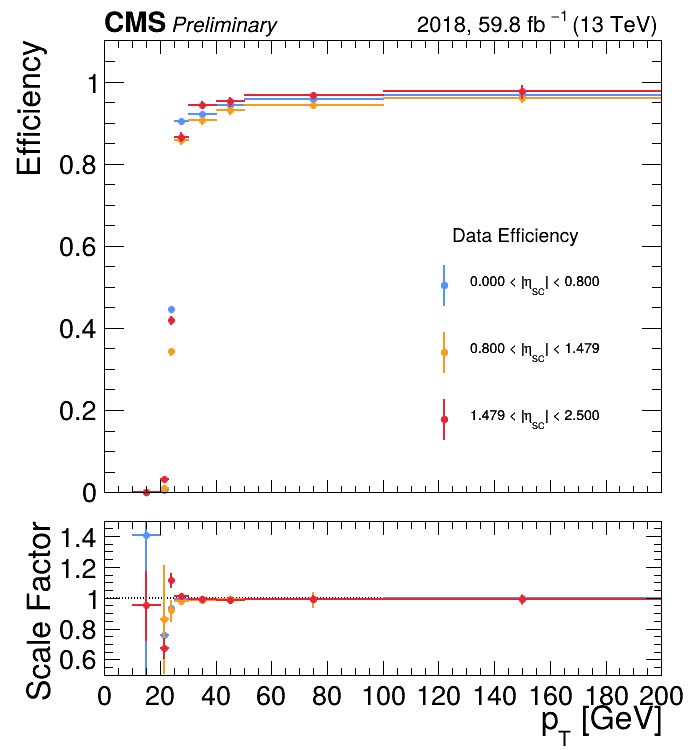
\includegraphics[width=0.23\textwidth]{Figures/analysis/Mu8El23_electron_eff_2018.png}}
  \caption{Leg efficiencies for the \texttt{Mu8\_El23} cross-trigger as functions of lepton $\pT$ in bins of $\eta$ or $\eta_\text{SC}$ for the Run~2 data-taking periods. The upper row shows the muon leg ($\pT > 8$\GeV), and the lower row shows the electron leg ($\pT > 23$\GeV).}
  \label{fig:trig_mu8el23_run2}
\end{sidewaysfigure}

\begin{sidewaysfigure}[p]
  \centering
  \subfloat[2022]{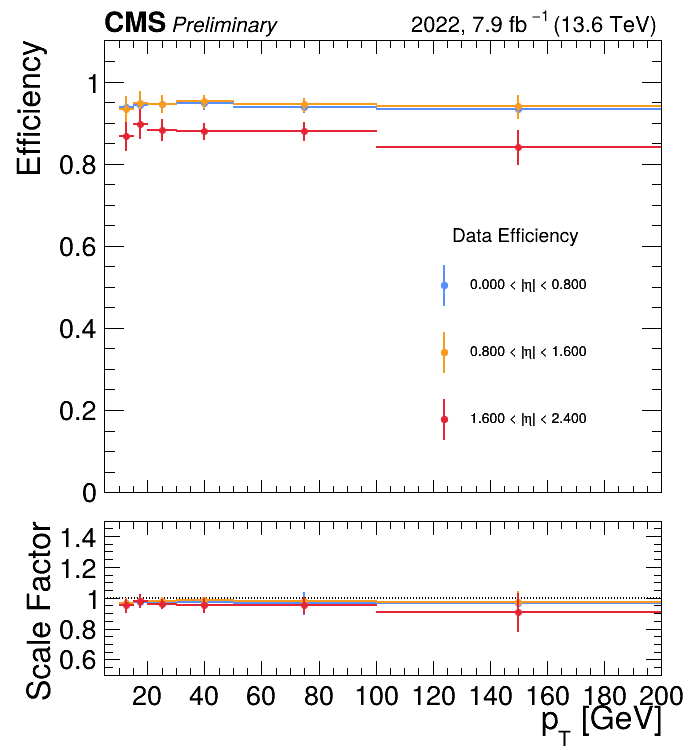
\includegraphics[width=0.23\textwidth]{Figures/analysis/Mu8El23_muon_eff_2022.png}}
  \hfill
  \subfloat[2022EE]{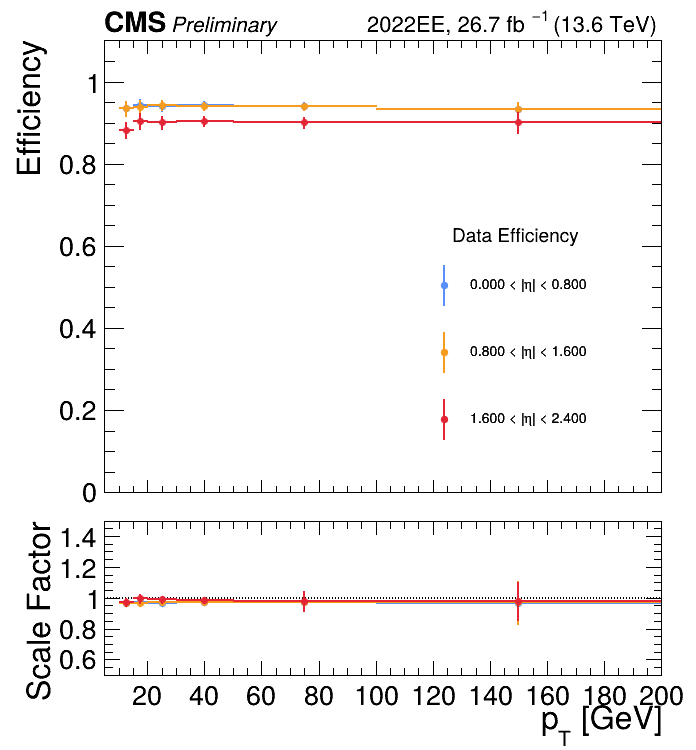
\includegraphics[width=0.23\textwidth]{Figures/analysis/Mu8El23_muon_eff_2022EE.png}}
  \hfill
  \subfloat[2023]{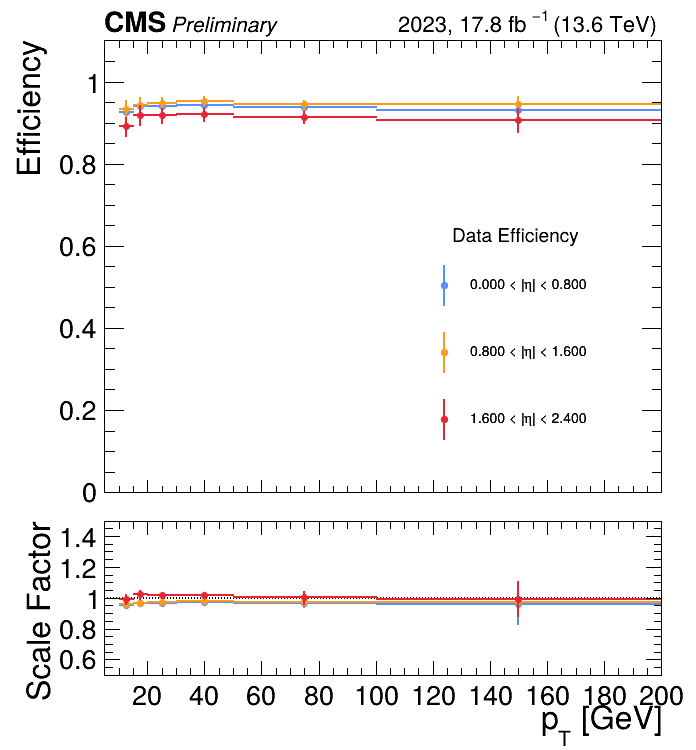
\includegraphics[width=0.23\textwidth]{Figures/analysis/Mu8El23_muon_eff_2023.png}}
  \hfill
  \subfloat[2023BPix]{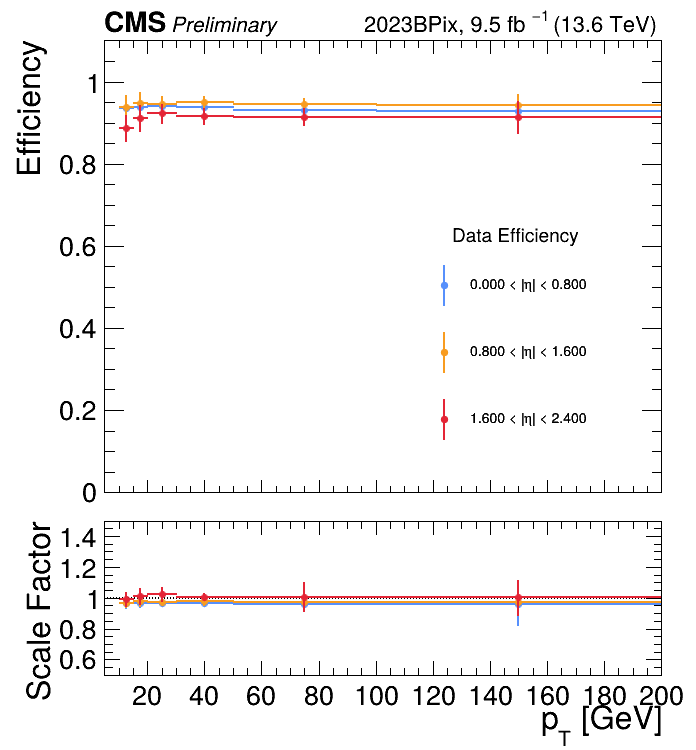
\includegraphics[width=0.23\textwidth]{Figures/analysis/Mu8El23_muon_eff_2023BPix.png}}
  \\
  \subfloat[2022]{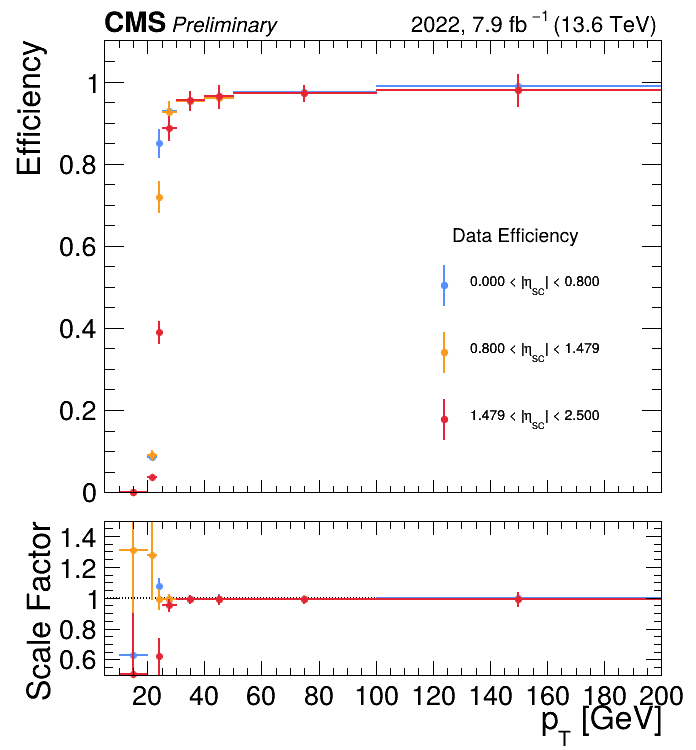
\includegraphics[width=0.23\textwidth]{Figures/analysis/Mu8El23_electron_eff_2022.png}}
  \hfill
  \subfloat[2022EE]{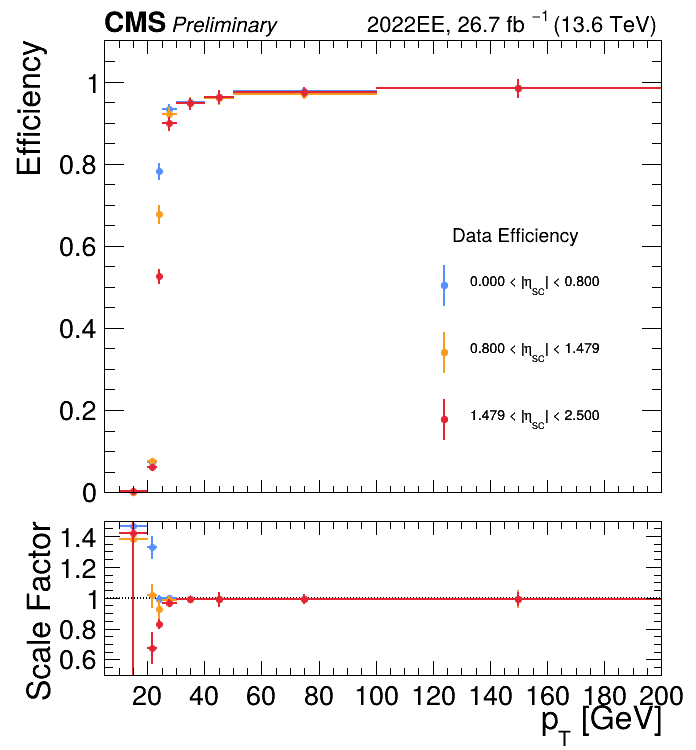
\includegraphics[width=0.23\textwidth]{Figures/analysis/Mu8El23_electron_eff_2022EE.png}}
  \hfill
  \subfloat[2023]{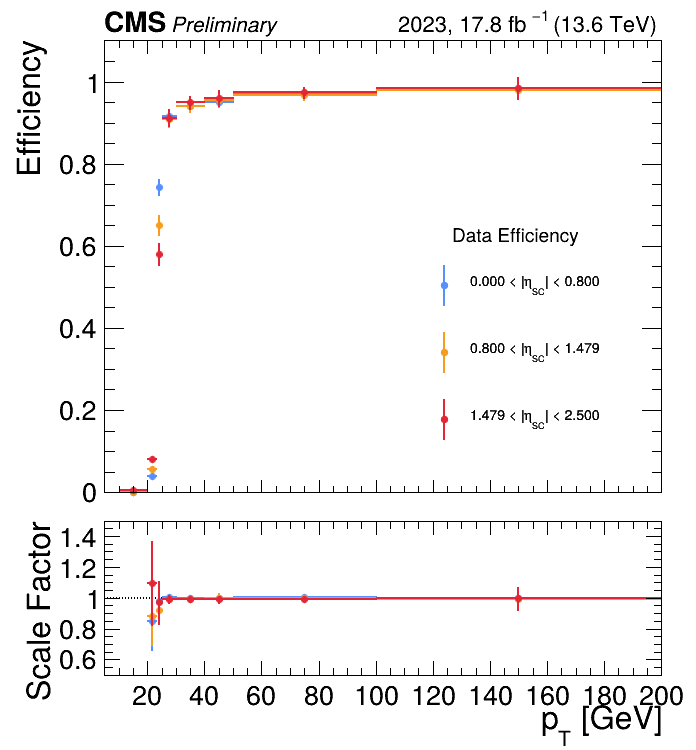
\includegraphics[width=0.23\textwidth]{Figures/analysis/Mu8El23_electron_eff_2023.png}}
  \hfill
  \subfloat[2023BPix]{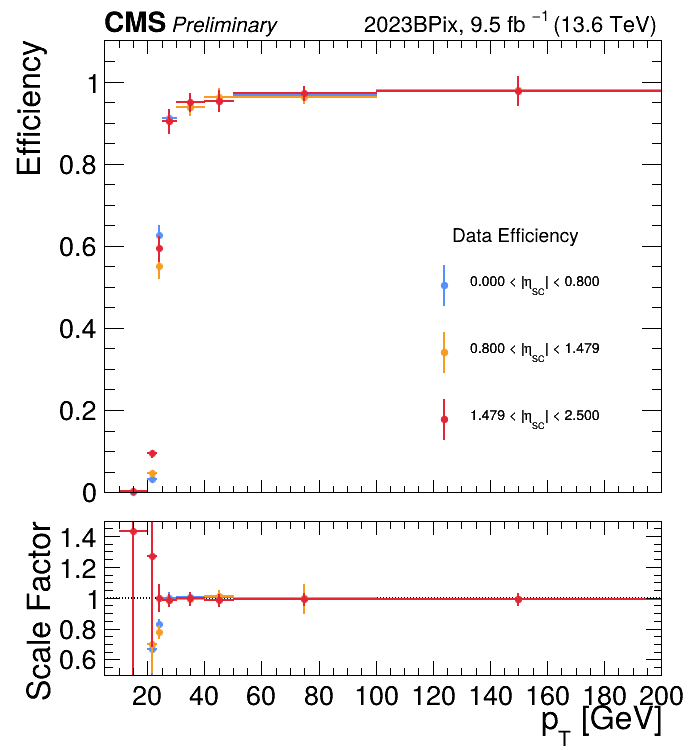
\includegraphics[width=0.23\textwidth]{Figures/analysis/Mu8El23_electron_eff_2023BPix.png}}
  \caption{Leg efficiencies for the \texttt{Mu8\_El23} cross-trigger as functions of lepton $\pT$ in bins of $\eta$ or $\eta_\text{SC}$ for the Run~3 data-taking periods. The upper row shows the muon leg ($\pT > 8$\GeV), and the lower row shows the electron leg ($\pT > 23$\GeV).}
  \label{fig:trig_mu8el23_run3}
\end{sidewaysfigure}

The pairwise filter efficiencies and their data-to-simulation scale factors are summarized in Tables~\ref{tab:pair_dimu} and~\ref{tab:pair_emu} for the dimuon and electron-muon triggers, respectively. In all cases the scale factors are consistent with unity at the sub-percent level.

\begin{table}[htbp]
\centering
\caption{Pairwise filter efficiency and data-to-simulation scale factor for dimuon triggers.}
\label{tab:pair_dimu}
\small
\begin{tabular}{llccc}
\hline\hline
Era & Filter & $\varepsilon_\text{data}$ & $\varepsilon_\text{MC}$ & SF \\
\hline
2016postVFP & DZ            & $0.9798 \pm 0.0006$ & $0.9968 \pm 0.0005$ & $0.9829 \pm 0.0008$ \\
2017 (B)     & DZ            & $0.9956 \pm 0.0009$ & $0.9958 \pm 0.0004$ & $0.9998 \pm 0.0010$ \\
2017 (C--F)  & DZ\_Mass3p8   & $0.9962 \pm 0.0012$ & $0.9958 \pm 0.0004$ & $1.0004 \pm 0.0013$ \\
2018         & DZ\_Mass3p8   & $0.9988 \pm 0.0011$ & $0.9998 \pm 0.0004$ & $0.9990 \pm 0.0012$ \\
2022         & DZ\_Mass3p8   & $0.9996 \pm 0.0029$ & $0.9998 \pm 0.0035$ & $0.9998 \pm 0.0046$ \\
2022EE       & DZ\_Mass3p8   & $0.9994 \pm 0.0017$ & $0.9998 \pm 0.0019$ & $0.9996 \pm 0.0026$ \\
2023         & DZ\_Mass3p8   & $0.9993 \pm 0.0019$ & $0.9997 \pm 0.0025$ & $0.9996 \pm 0.0032$ \\
2023BPix     & DZ\_Mass3p8   & $0.9989 \pm 0.0026$ & $0.9996 \pm 0.0035$ & $0.9993 \pm 0.0044$ \\
\hline\hline
\end{tabular}
\end{table}

\begin{table}[htbp]
\centering
\caption{Pairwise filter efficiency and data-to-simulation scale factor for electron-muon triggers.}
\label{tab:pair_emu}
\small
\begin{tabular}{llccc}
\hline\hline
Era & Filter & $\varepsilon_\text{data}$ & $\varepsilon_\text{MC}$ & SF \\
\hline
2016postVFP & DZ & $0.9638 \pm 0.0037$ & $0.9878 \pm 0.0007$ & $0.9757 \pm 0.0038$ \\
2017         & DZ & $0.9989 \pm 0.0023$ & $0.9955 \pm 0.0004$ & $1.0034 \pm 0.0023$ \\
2018         & DZ & $0.9946 \pm 0.0018$ & $0.9981 \pm 0.0004$ & $0.9965 \pm 0.0018$ \\
2022         & DZ & $0.9964 \pm 0.0048$ & $0.9985 \pm 0.0010$ & $0.9979 \pm 0.0049$ \\
2022EE       & DZ & $0.9949 \pm 0.0028$ & $0.9976 \pm 0.0006$ & $0.9973 \pm 0.0029$ \\
2023         & DZ & $0.9944 \pm 0.0032$ & $0.9977 \pm 0.0008$ & $0.9967 \pm 0.0033$ \\
2023BPix     & DZ & $0.9930 \pm 0.0044$ & $0.9972 \pm 0.0011$ & $0.9958 \pm 0.0045$ \\
\hline\hline
\end{tabular}
\end{table}

\subsubsection*{Jet energy corrections and b-tagging scale factors}

The JES and JER corrections described in Section~\ref{ssec:jets} use the latest calibrations provided by the JMET POG for each data-taking era. Systematic uncertainties are evaluated by varying the corrections within their uncertainties and propagating the effect to the final observable.

Flavor-dependent b-tagging scale factors from the BTV POG are applied on a per-jet basis using the fixed working point method (method 1a)~\cite{CMS:2017wtu}. The scale factors are derived from QCD multijet events and correct for differences in the b-tagging efficiency between data and simulation separately for b~quarks, c~quarks, and light-flavor jets.

\subsubsection*{Pileup reweighting}

The distribution of pileup interactions in simulation is reweighted to match the observed pileup profile in data, as described in Section~\ref{ssec:mc_samples}. The minimum bias cross section used in the pileup calculation is varied within its uncertainty to evaluate the associated systematic effect.

\subsection{Validation of object corrections}
\label{ssec:validation}

The combined effect of the object identification, trigger efficiency, jet energy, b-tagging, and pileup corrections described in the preceding subsections is validated in two dilepton control regions, chosen to probe the dominant physics objects in the analysis while remaining orthogonal to the trilepton signal region.

\subsubsection*{Inclusive dimuon control region}

Inclusive di-muon events are selected by requiring events to pass the dimuon triggers (Section~\ref{ssec:triggers}), contain exactly two opposite-charge muons satisfying the tight working point with $\pT > 20$\GeV and $10$\GeV for the leading and subleading muon, no additional loose leptons, and a dimuon invariant mass $m(\Pgm\Pgm) > 50$\GeV. This region is dominated by Drell--Yan production and validates the muon identification and isolation scale factors, the Rochester momentum corrections, the dimuon trigger efficiency, and the pileup reweighting.

The muon $\pT$ and $\eta$ distributions, the dimuon invariant mass, and the number of primary vertices are shown in Fig.~\ref{fig:dimu_cr}. The simulation, with all corrections applied, describes the data within the systematic uncertainty band across all kinematic variables.

\begin{figure}[p]
  \centering
  \subfloat{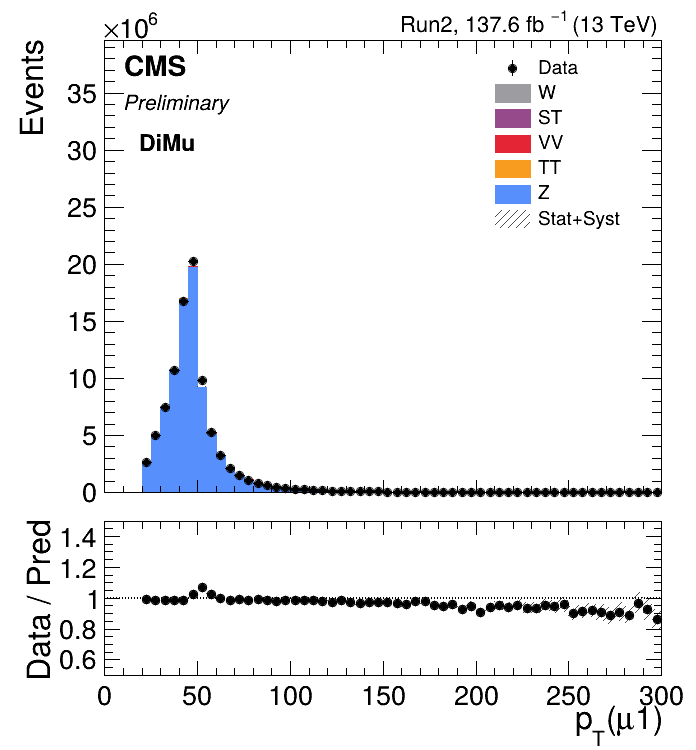
\includegraphics[width=0.26\textwidth]{Figures/analysis/DiMu_Run2_muons_1_pt.png}}
  \subfloat{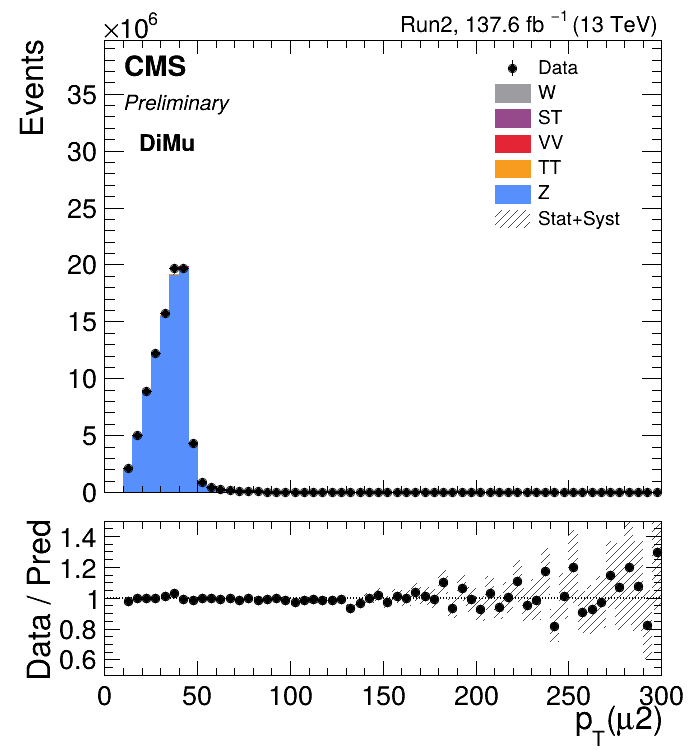
\includegraphics[width=0.26\textwidth]{Figures/analysis/DiMu_Run2_muons_2_pt.png}}
  \subfloat{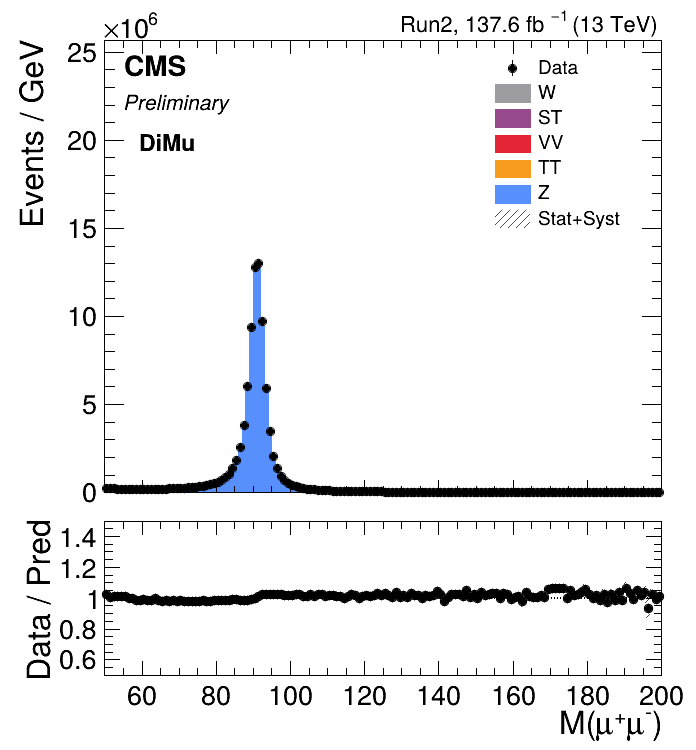
\includegraphics[width=0.26\textwidth]{Figures/analysis/DiMu_Run2_pair_mass.png}} \\
  \subfloat{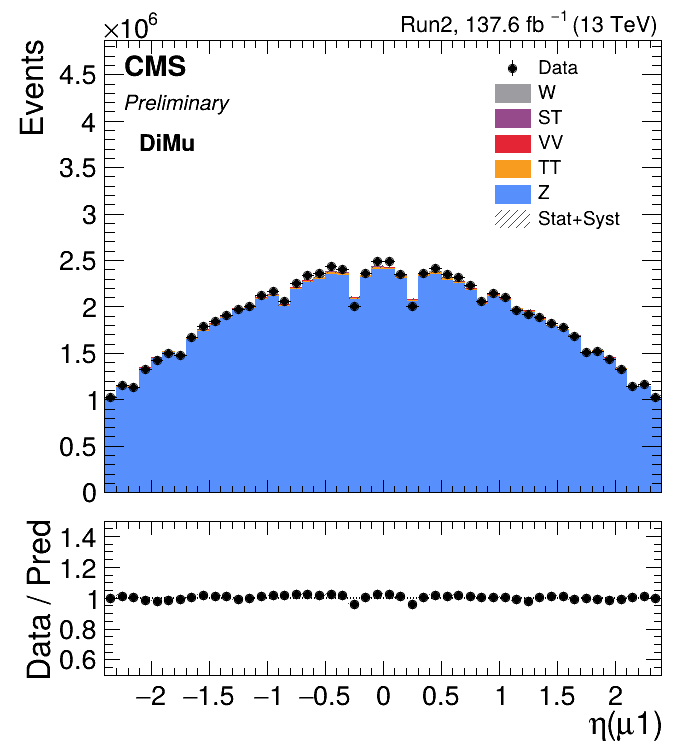
\includegraphics[width=0.26\textwidth]{Figures/analysis/DiMu_Run2_muons_1_eta.png}}
  \subfloat{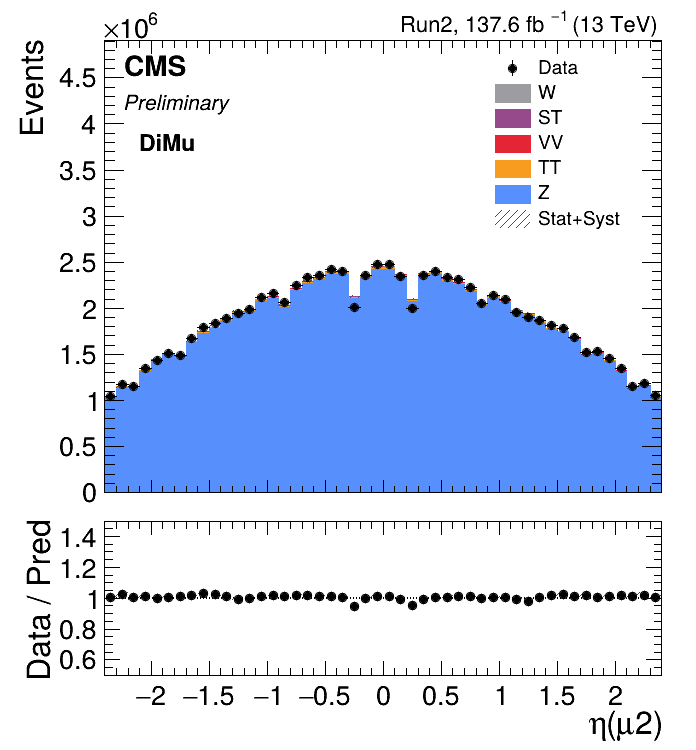
\includegraphics[width=0.26\textwidth]{Figures/analysis/DiMu_Run2_muons_2_eta.png}}
  \subfloat{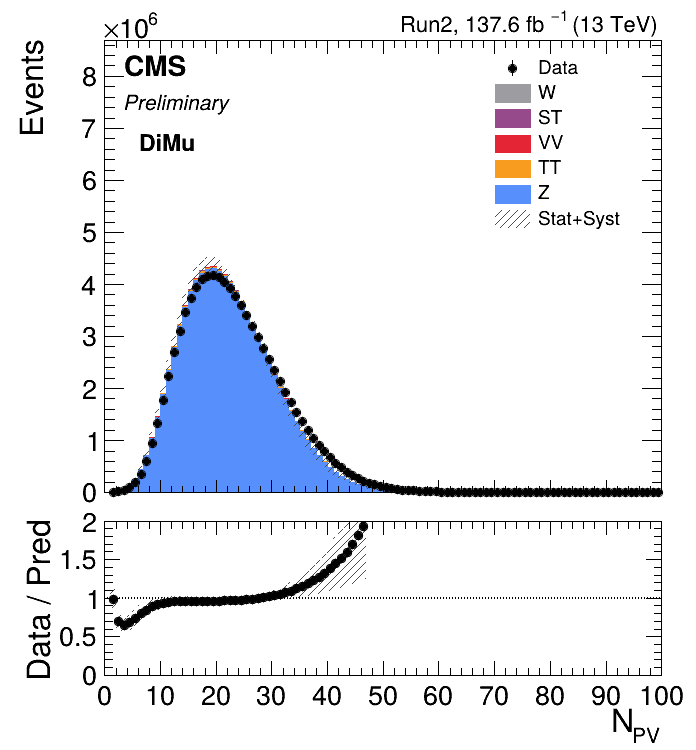
\includegraphics[width=0.26\textwidth]{Figures/analysis/DiMu_Run2_nPVsGood.png}} \\
  \subfloat{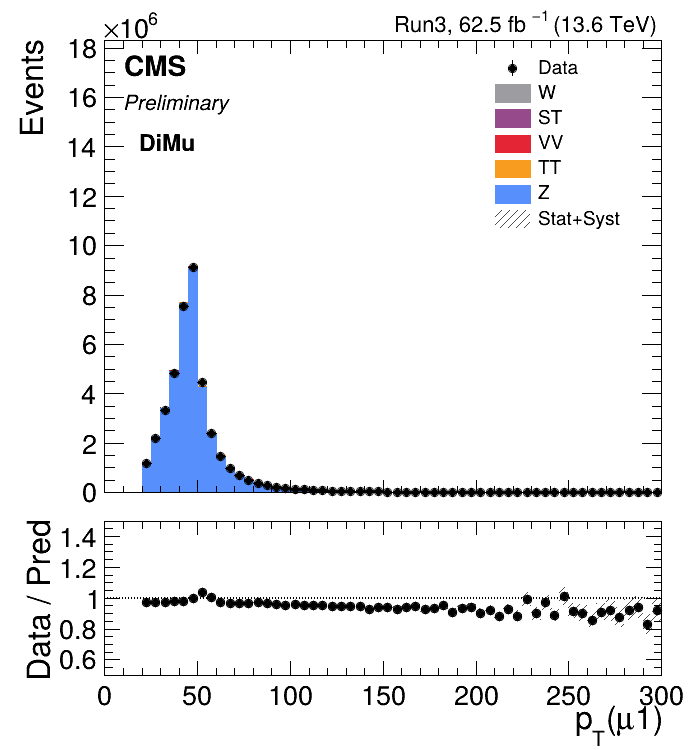
\includegraphics[width=0.26\textwidth]{Figures/analysis/DiMu_Run3_muons_1_pt.png}}
  \subfloat{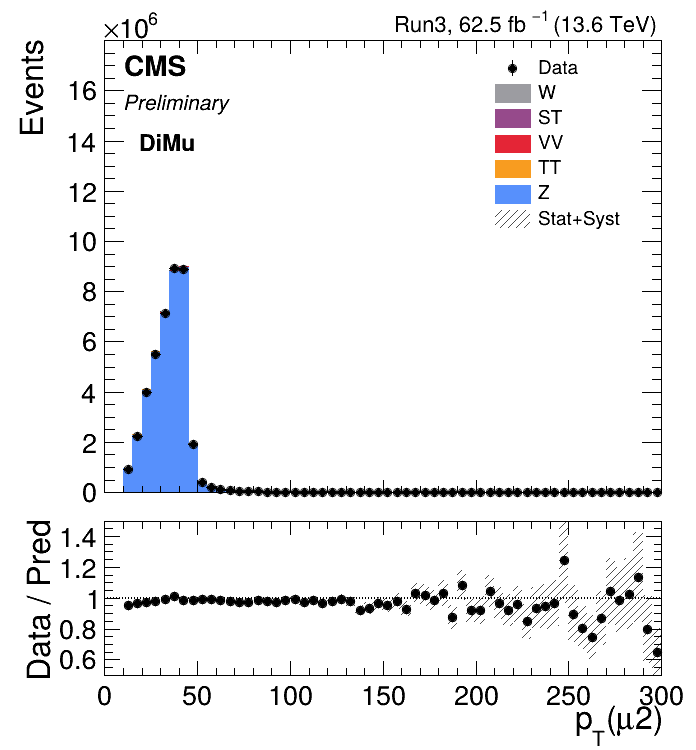
\includegraphics[width=0.26\textwidth]{Figures/analysis/DiMu_Run3_muons_2_pt.png}}
  \subfloat{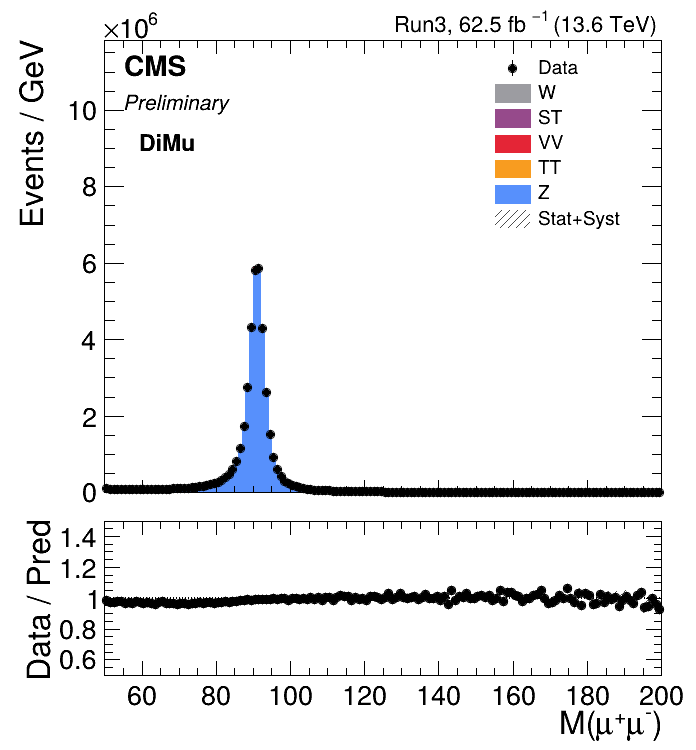
\includegraphics[width=0.26\textwidth]{Figures/analysis/DiMu_Run3_pair_mass.png}} \\
  \subfloat{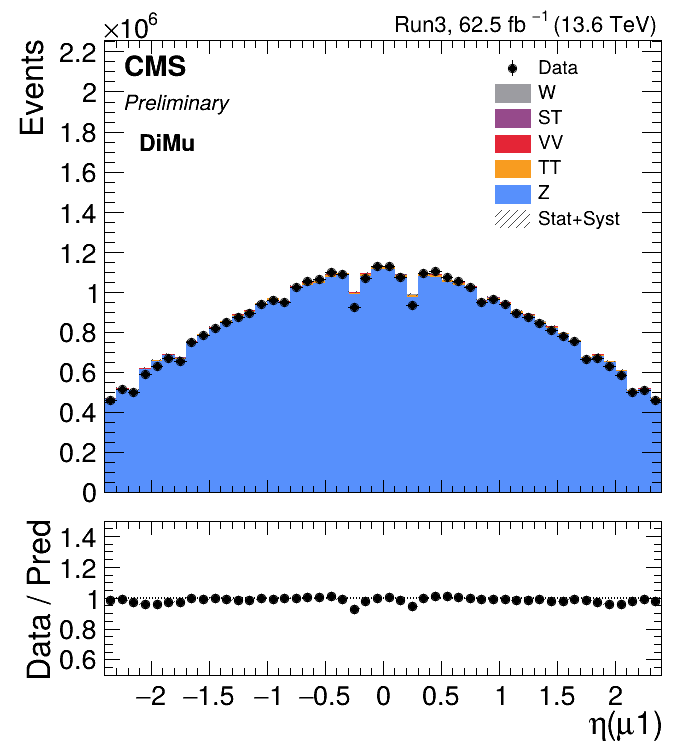
\includegraphics[width=0.26\textwidth]{Figures/analysis/DiMu_Run3_muons_1_eta.png}}
  \subfloat{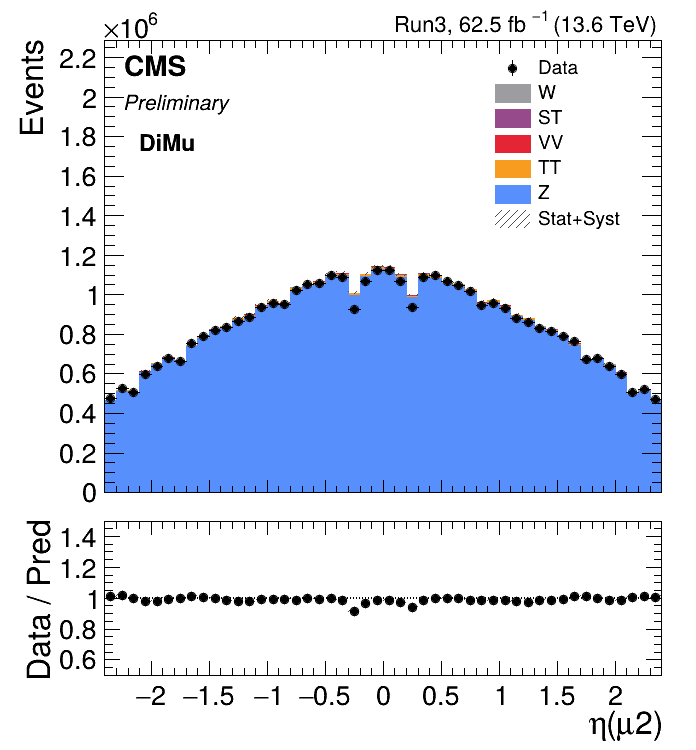
\includegraphics[width=0.26\textwidth]{Figures/analysis/DiMu_Run3_muons_2_eta.png}}
  \subfloat{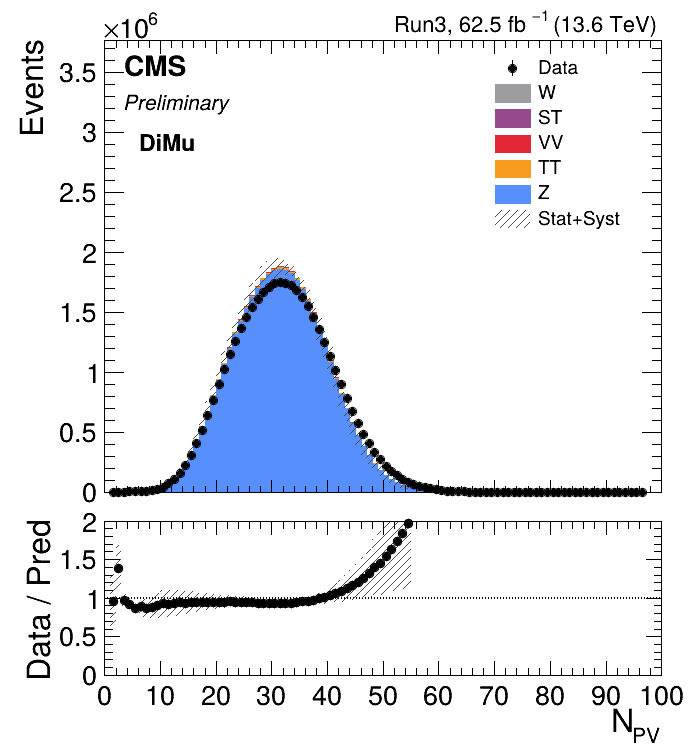
\includegraphics[width=0.26\textwidth]{Figures/analysis/DiMu_Run3_nPVsGood.png}}
  \caption{Distributions of the leading and subleading muon $\pT$ and $\eta$, the dimuon invariant mass, and the number of reconstructed primary vertices in the inclusive dimuon control region for Run~2 (rows~1--2) and Run~3 (rows~3--4). The hatched band represents the combined statistical and systematic uncertainty on the prediction.}
  \label{fig:dimu_cr}
\end{figure}

\subsubsection*{Top-enriched electron-muon control region}

A $\ttbar$-enriched $\Pe\Pgm$ sample is selected by requiring events to pass the electron-muon cross-triggers, contain exactly one opposite-charge electron-muon pair satisfying $\pT(\Pgm) > 25$\GeV and $\pT(\Pe) > 15$\GeV, or $\pT(\Pgm) > 10$\GeV and $\pT(\Pe) > 25$\GeV, with $\Delta R(\Pe, \Pgm) > 0.4$, no additional loose leptons, and at least two jets with at least one b-tagged jet. This region validates the electron identification and isolation scale factors, the electron-muon trigger efficiency, the jet energy corrections, and the b-tagging scale factors in a topology enriched in genuine $\ptmiss$ from $\PW$ boson decays.

The lepton $\pT$, $\eta$, $\ptmiss$, and pileup distributions are shown in Fig.~\ref{fig:emu_cr_lep}, and the jet and b-jet kinematic and multiplicity distributions in Fig.~\ref{fig:emu_cr_jet}. Good agreement between data and simulation is observed across all distributions for both Run~2 and Run~3.

\begin{figure}[p]
  \centering
  \subfloat{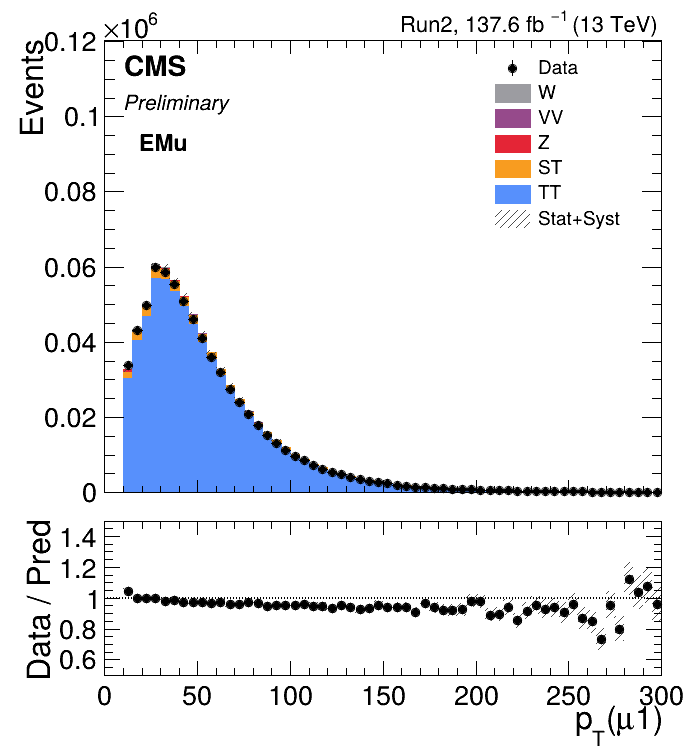
\includegraphics[width=0.26\textwidth]{Figures/analysis/EMu_Run2_muons_1_pt.png}}
  \subfloat{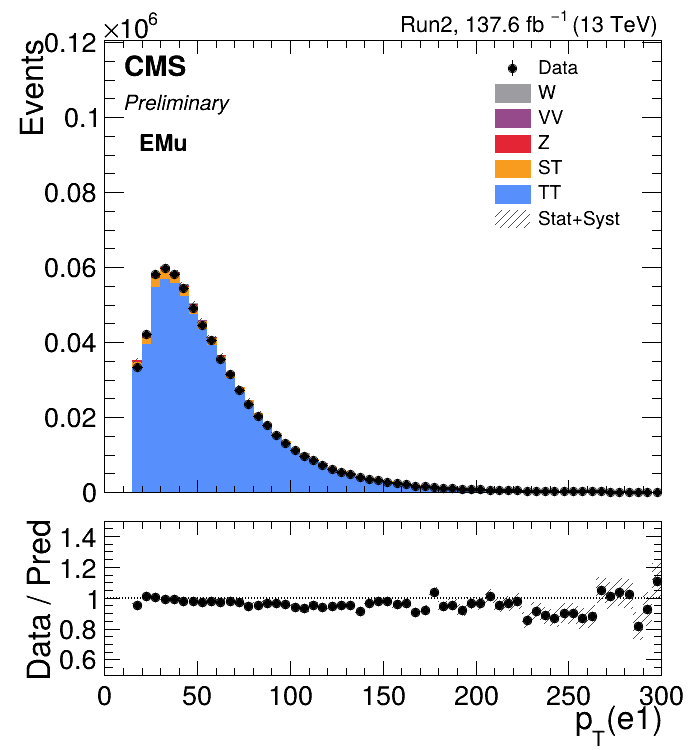
\includegraphics[width=0.26\textwidth]{Figures/analysis/EMu_Run2_electrons_1_pt.png}}
  \subfloat{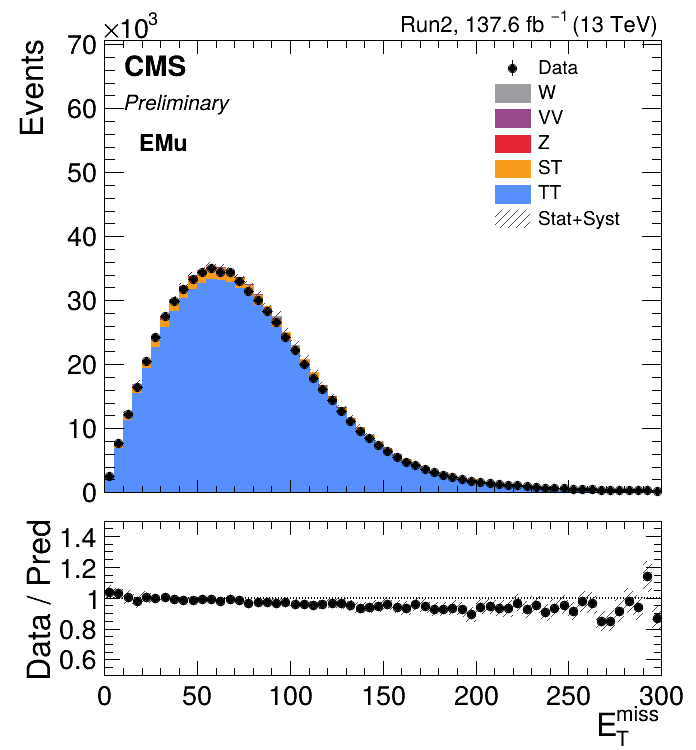
\includegraphics[width=0.26\textwidth]{Figures/analysis/EMu_Run2_METv_pt.png}} \\
  \subfloat{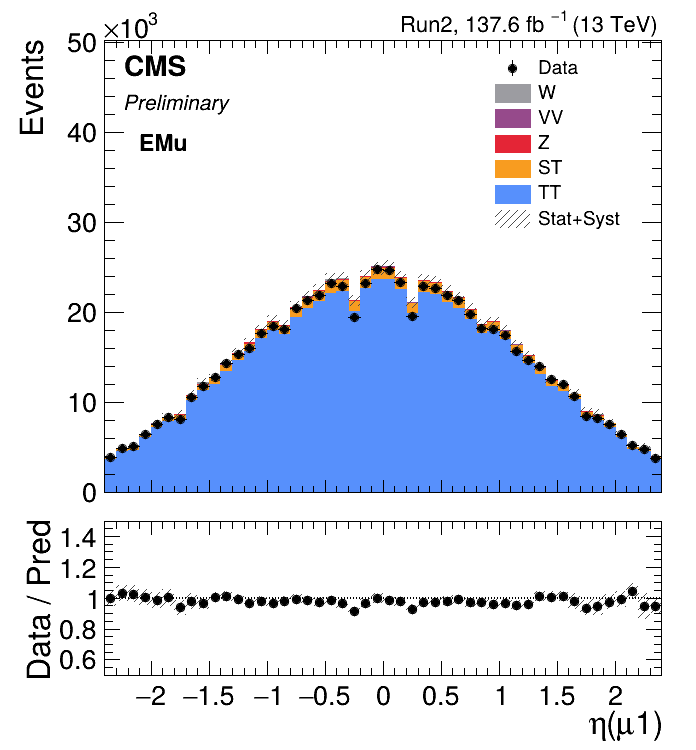
\includegraphics[width=0.26\textwidth]{Figures/analysis/EMu_Run2_muons_1_eta.png}}
  \subfloat{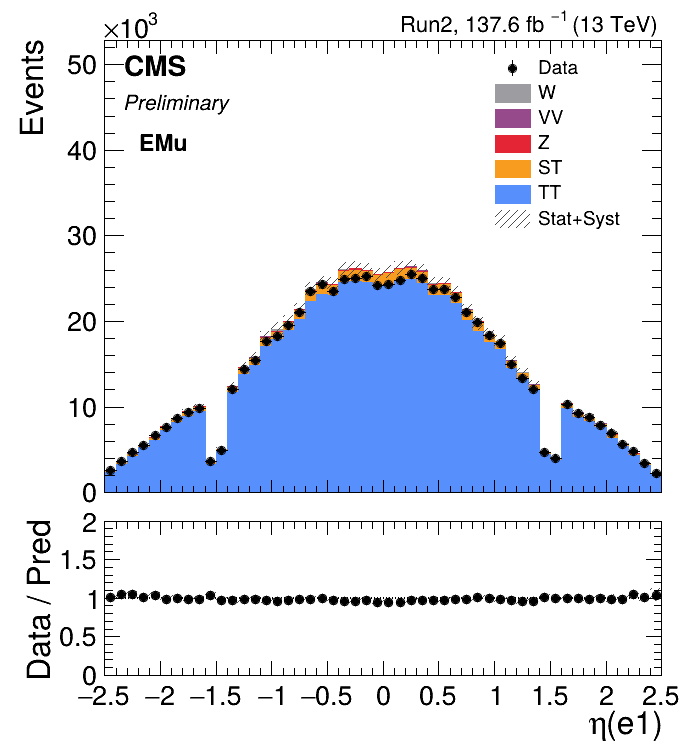
\includegraphics[width=0.26\textwidth]{Figures/analysis/EMu_Run2_electrons_1_eta.png}}
  \subfloat{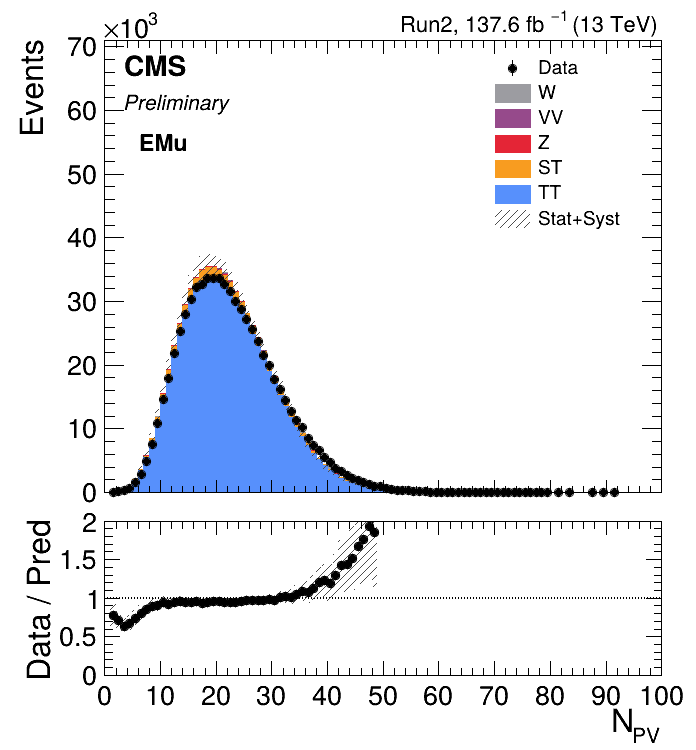
\includegraphics[width=0.26\textwidth]{Figures/analysis/EMu_Run2_nPVsGood.png}} \\
  \subfloat{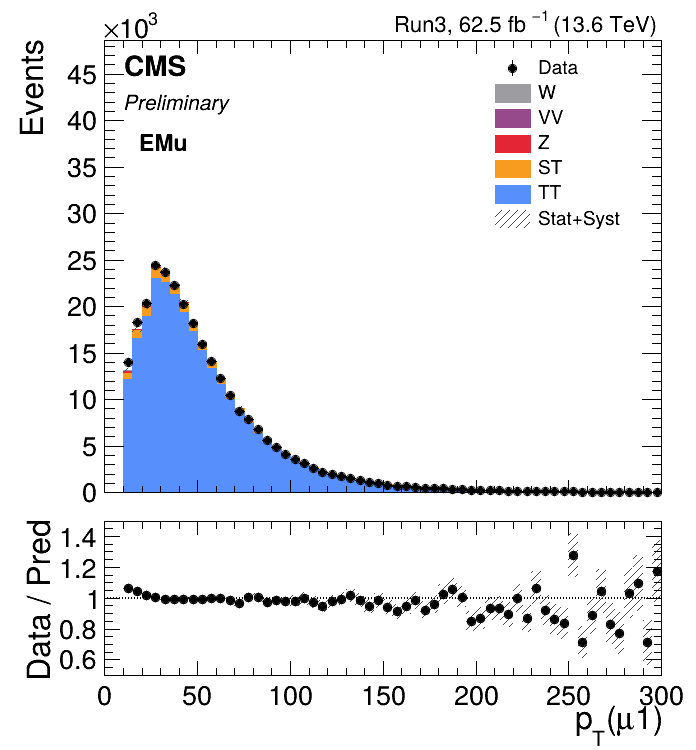
\includegraphics[width=0.26\textwidth]{Figures/analysis/EMu_Run3_muons_1_pt.png}}
  \subfloat{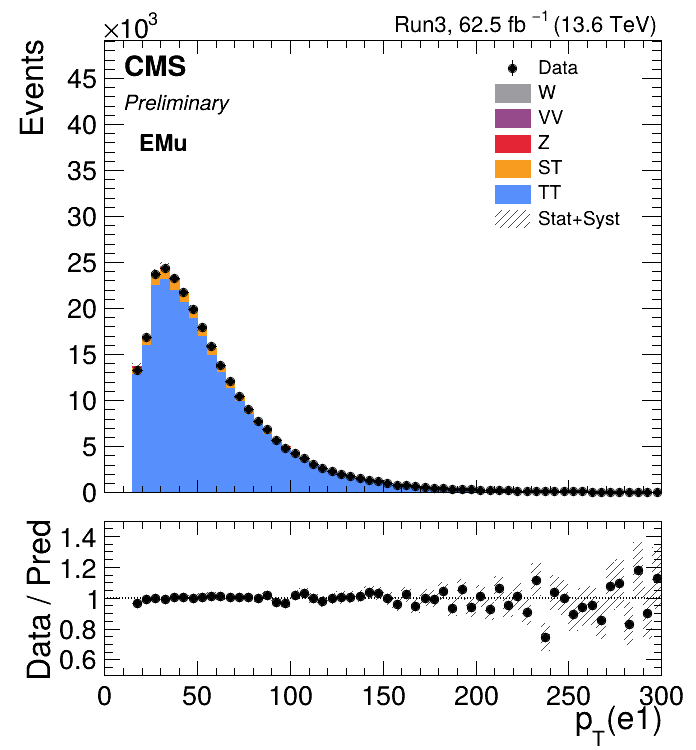
\includegraphics[width=0.26\textwidth]{Figures/analysis/EMu_Run3_electrons_1_pt.png}}
  \subfloat{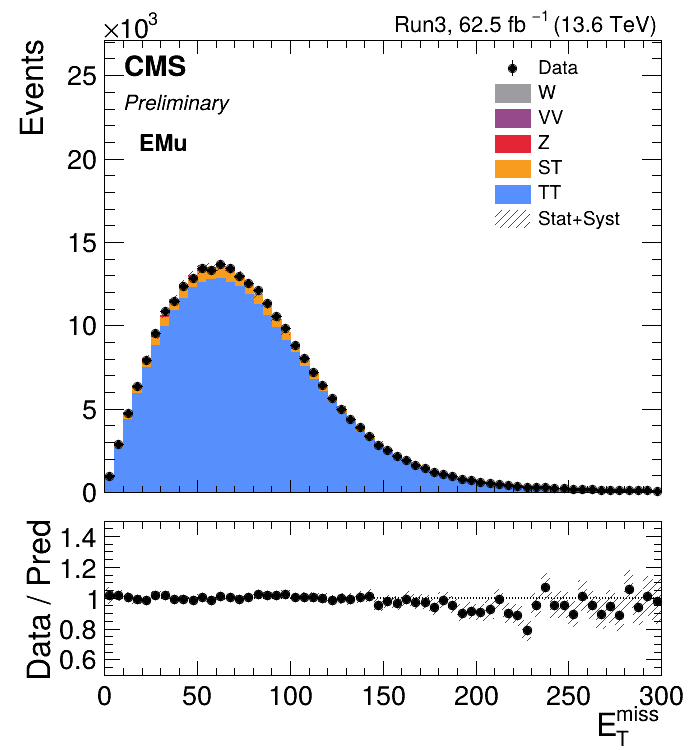
\includegraphics[width=0.26\textwidth]{Figures/analysis/EMu_Run3_METv_pt.png}} \\
  \subfloat{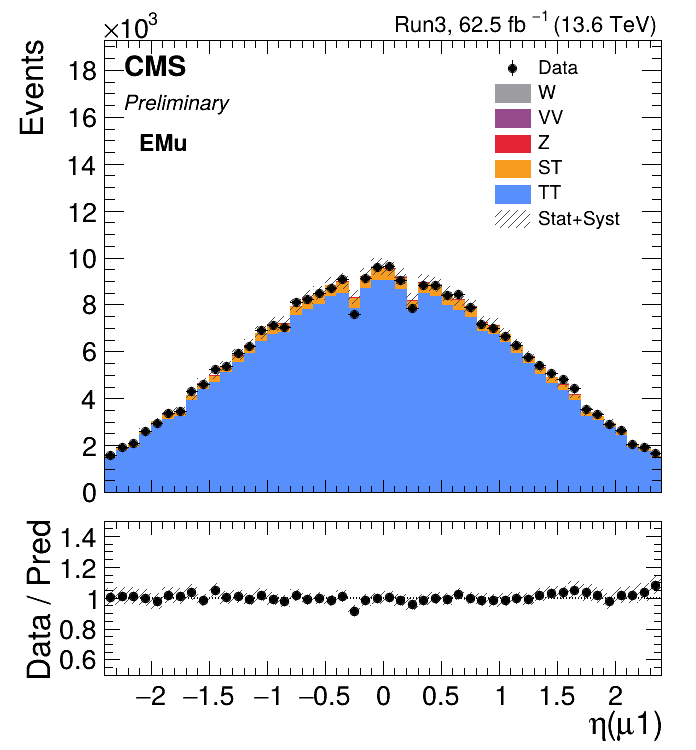
\includegraphics[width=0.26\textwidth]{Figures/analysis/EMu_Run3_muons_1_eta.png}}
  \subfloat{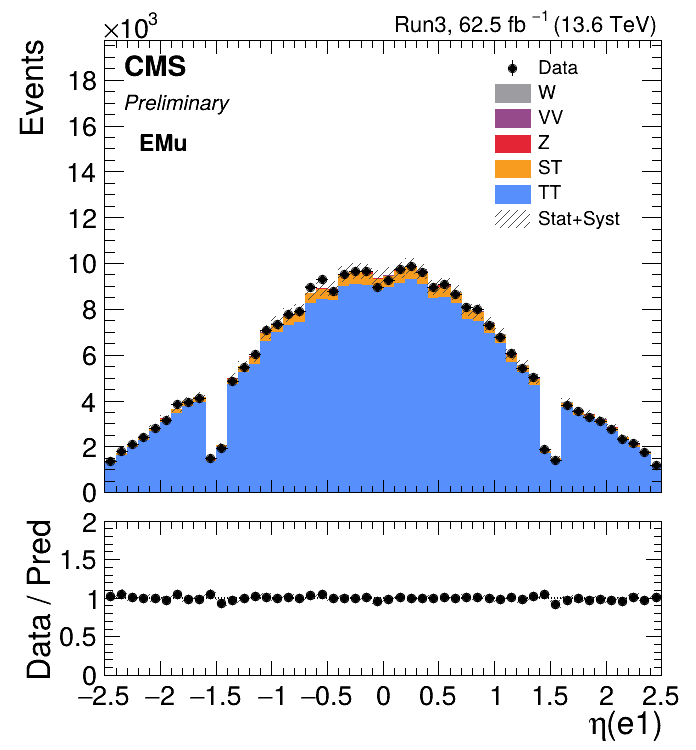
\includegraphics[width=0.26\textwidth]{Figures/analysis/EMu_Run3_electrons_1_eta.png}}
  \subfloat{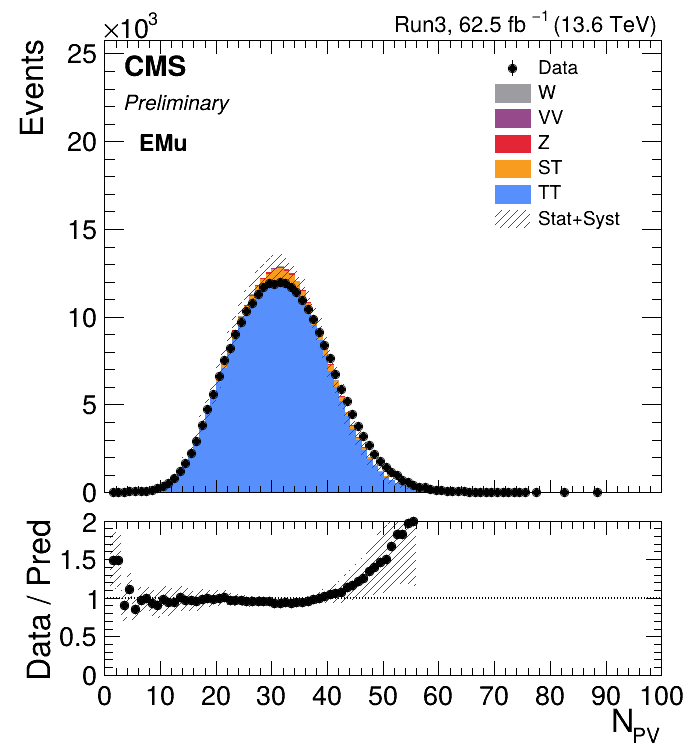
\includegraphics[width=0.26\textwidth]{Figures/analysis/EMu_Run3_nPVsGood.png}}
  \caption{Distributions of lepton $\pT$ and $\eta$, $\ptmiss$, and the number of reconstructed primary vertices in the top-enriched $\Pe\Pgm$ control region for Run~2 (rows~1--2) and Run~3 (rows~3--4).}
  \label{fig:emu_cr_lep}
\end{figure}

\begin{figure}[p]
  \centering
  \subfloat{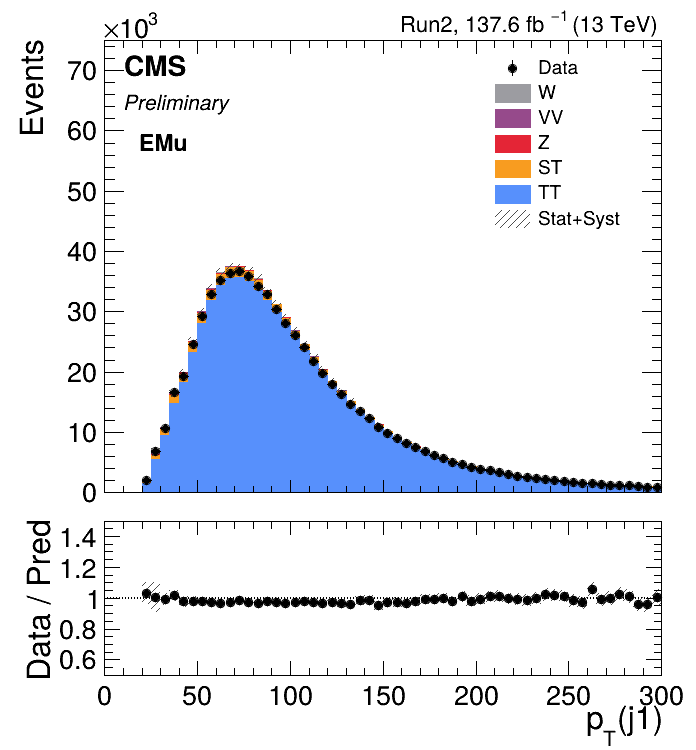
\includegraphics[width=0.26\textwidth]{Figures/analysis/EMu_Run2_jets_1_pt.png}}
  \subfloat{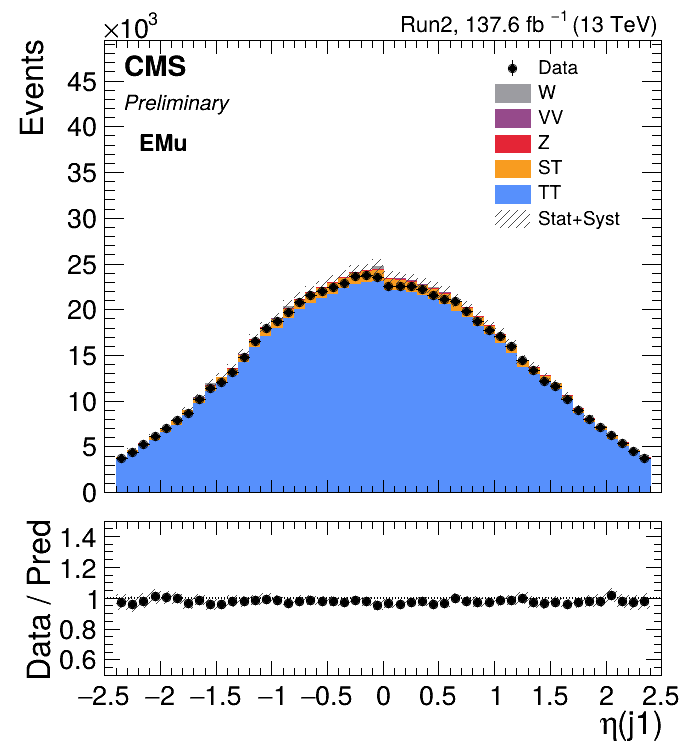
\includegraphics[width=0.26\textwidth]{Figures/analysis/EMu_Run2_jets_1_eta.png}}
  \subfloat{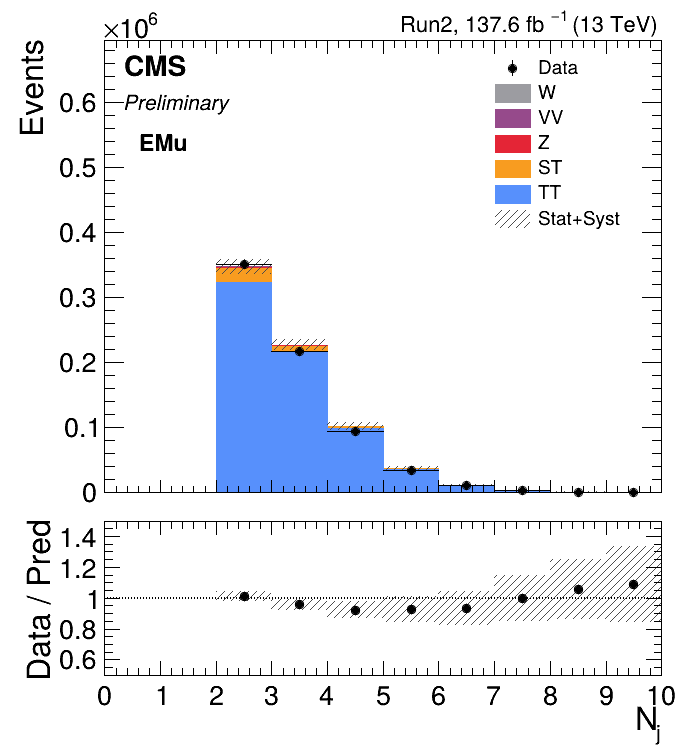
\includegraphics[width=0.26\textwidth]{Figures/analysis/EMu_Run2_jets_size.png}} \\
  \subfloat{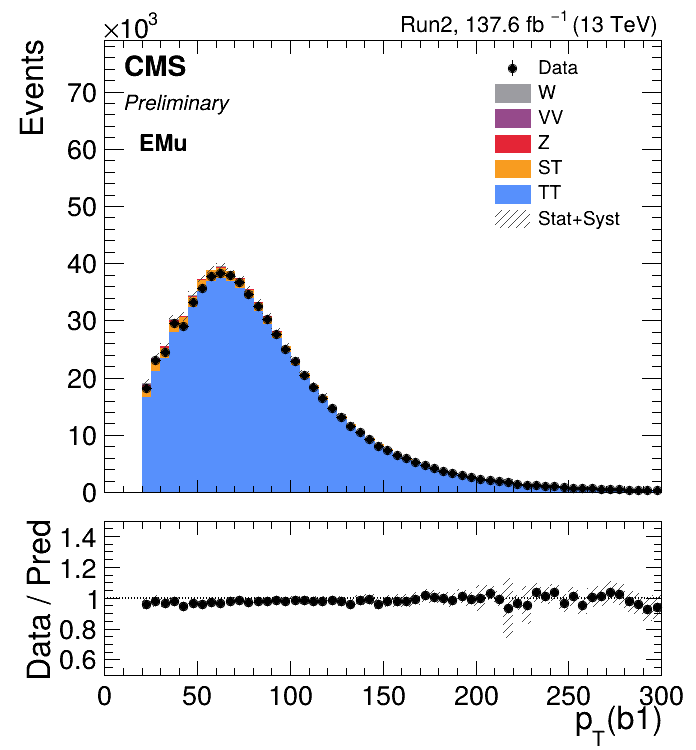
\includegraphics[width=0.26\textwidth]{Figures/analysis/EMu_Run2_bjets_1_pt.png}}
  \subfloat{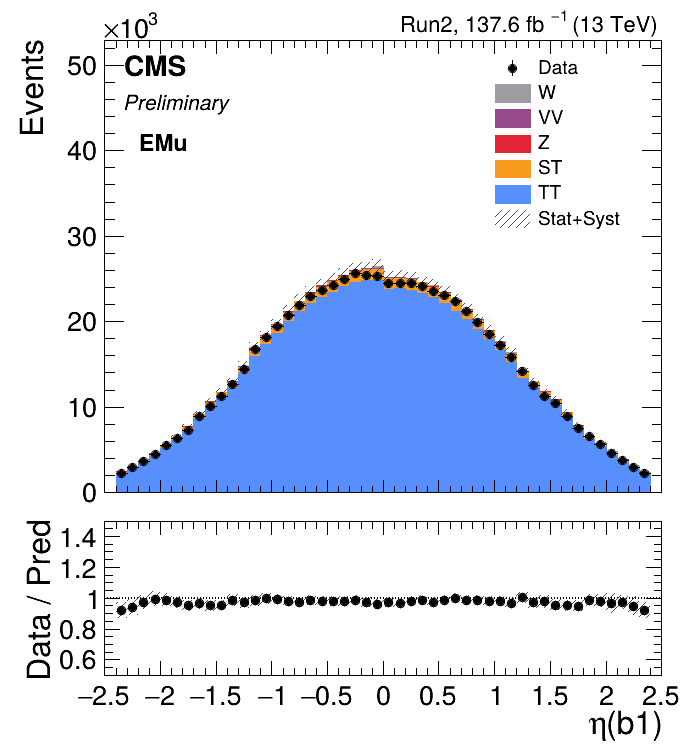
\includegraphics[width=0.26\textwidth]{Figures/analysis/EMu_Run2_bjets_1_eta.png}}
  \subfloat{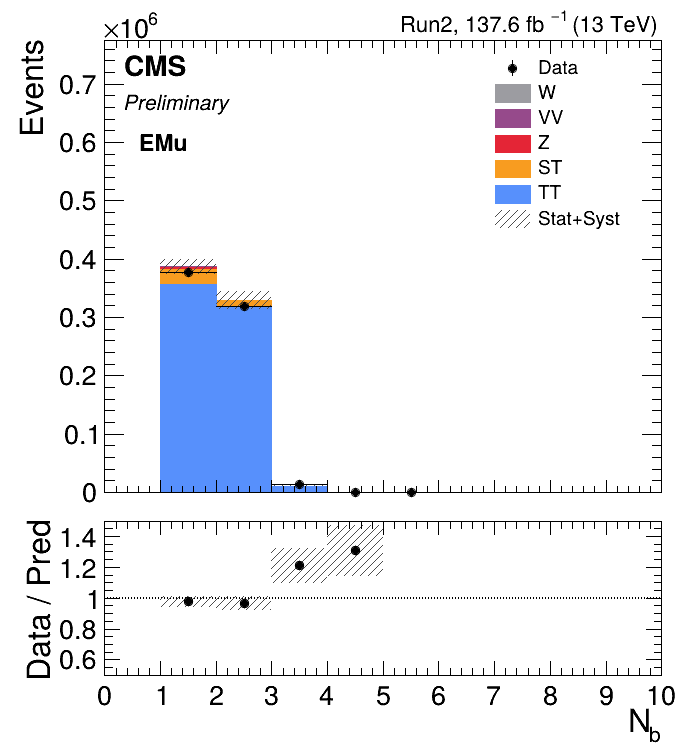
\includegraphics[width=0.26\textwidth]{Figures/analysis/EMu_Run2_bjets_size.png}} \\
  \subfloat{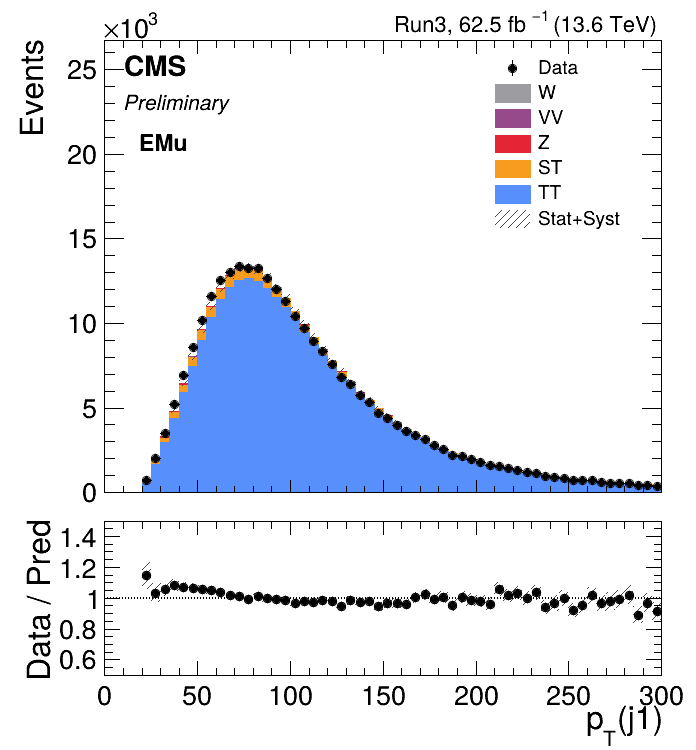
\includegraphics[width=0.26\textwidth]{Figures/analysis/EMu_Run3_jets_1_pt.png}}
  \subfloat{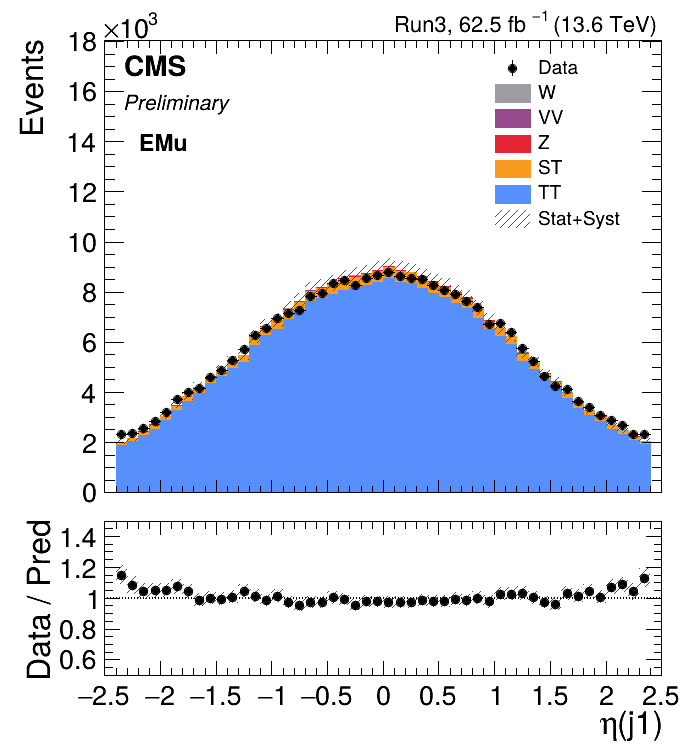
\includegraphics[width=0.26\textwidth]{Figures/analysis/EMu_Run3_jets_1_eta.png}}
  \subfloat{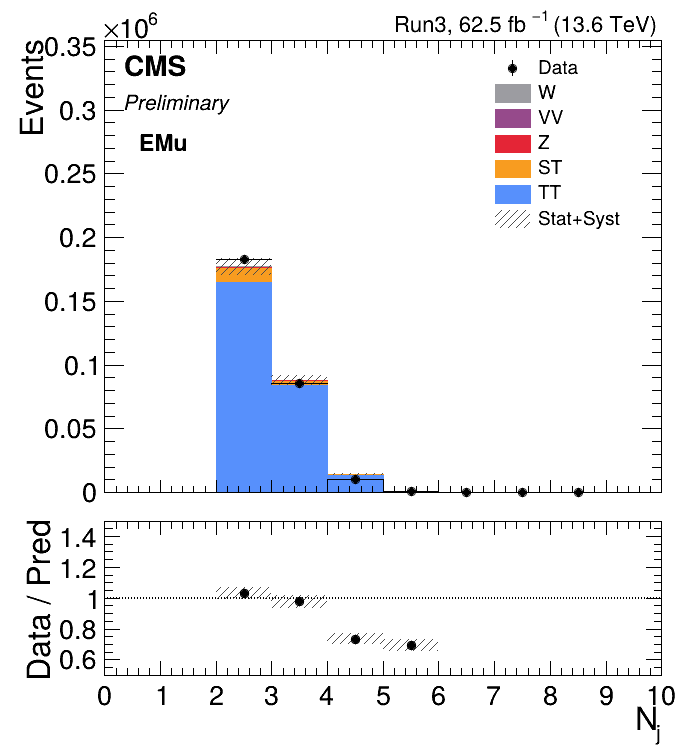
\includegraphics[width=0.26\textwidth]{Figures/analysis/EMu_Run3_jets_size.png}} \\
  \subfloat{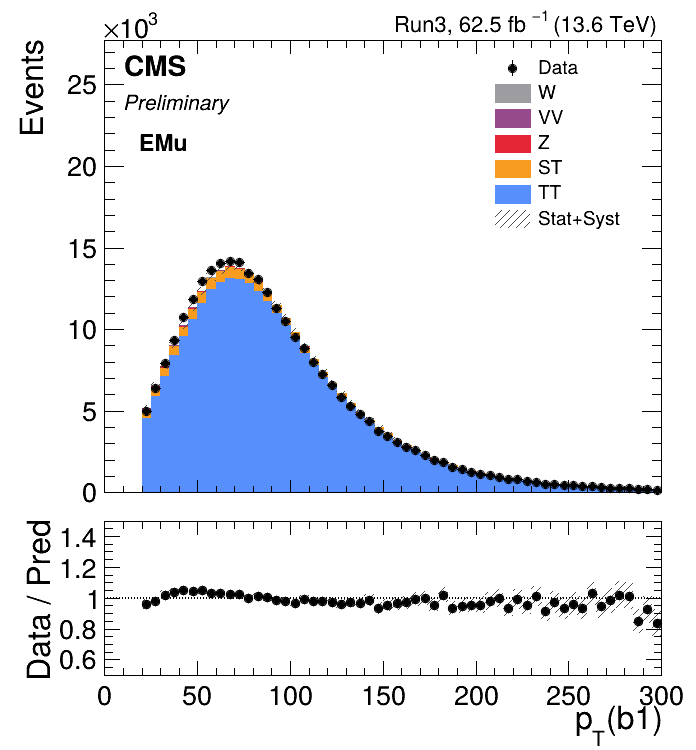
\includegraphics[width=0.26\textwidth]{Figures/analysis/EMu_Run3_bjets_1_pt.png}}
  \subfloat{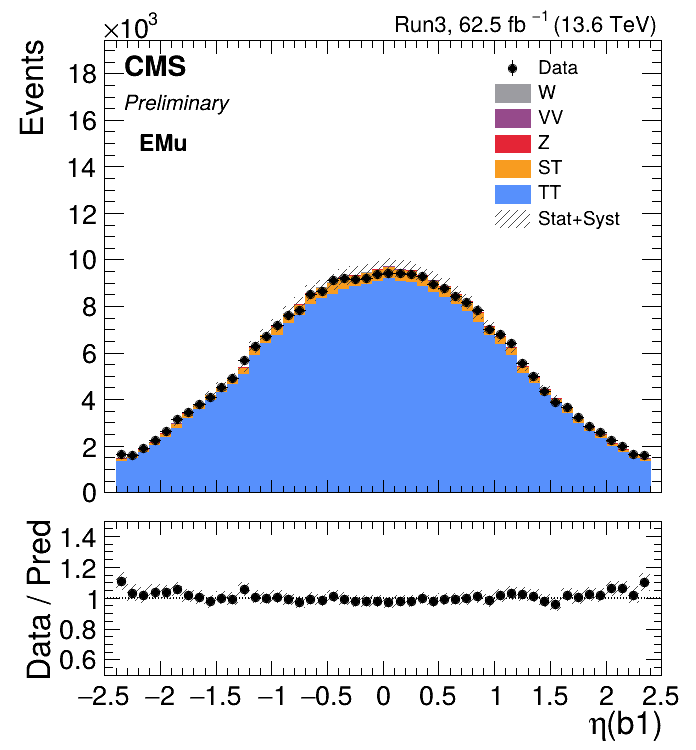
\includegraphics[width=0.26\textwidth]{Figures/analysis/EMu_Run3_bjets_1_eta.png}}
  \subfloat{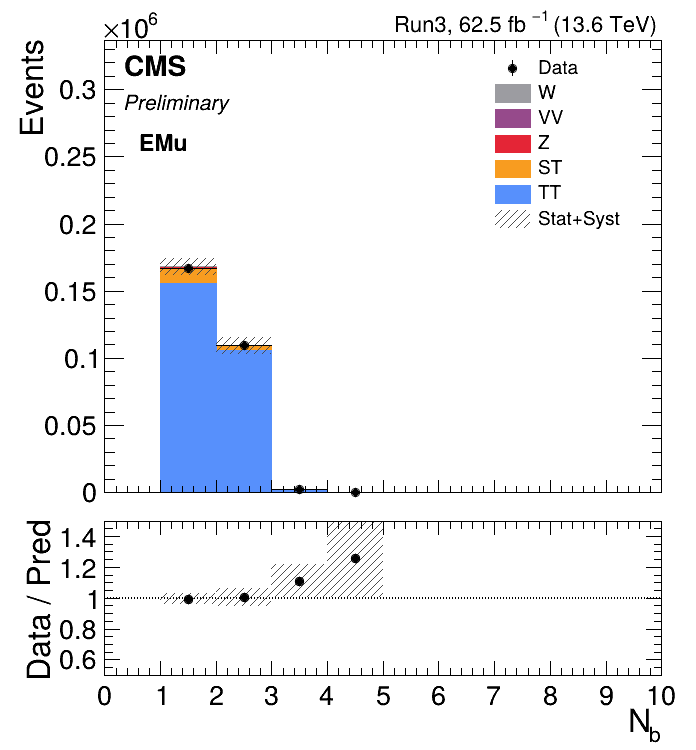
\includegraphics[width=0.26\textwidth]{Figures/analysis/EMu_Run3_bjets_size.png}}
  \caption{Distributions of leading jet and leading b-tagged jet $\pT$, $\eta$, and multiplicity in the top-enriched $\Pe\Pgm$ control region for Run~2 (rows~1--2) and Run~3 (rows~3--4).}
  \label{fig:emu_cr_jet}
\end{figure}
